\documentclass[modern]{aastex62}

\usepackage{color}
\usepackage{amsmath}
\usepackage{enumitem}
\usepackage{graphicx}
\usepackage{mathrsfs}
\usepackage{booktabs}
\usepackage{morefloats}

% \usepackage{draftwatermark}
% \SetWatermarkScale{3}
% \SetWatermarkLightness{.7}

\newcommand{\code}[1]{\texttt{\detokenize{#1}}}
\newcommand{\apogee}{\textsl{APOGEE}}
\newcommand{\thecannon}{\textsl{The Cannon}}
\newcommand{\cannon}{\textsl{Cannon}}
\newcommand{\aspcap}{\textsl{ASPCAP}}
\newcommand{\gaia}{\textsl{Gaia}}
\newcommand{\zmass}{\textsl{2MASS}}
\newcommand{\sdss}{\textsl{SDSS}}
\newcommand{\kepler}{\textsl{Kepler}}
\newcommand{\lamost}{\textsl{LAMOST}}
\newcommand{\sdssiv}{\textsl{SDSS-IV}}
\newcommand{\tess}{\textsl{TESS}}
\newcommand{\msun}{M_{\odot}}
\newcommand{\teff}{T_{\mathrm{eff}}}
\newcommand{\logg}{\log g}
\newcommand{\feh}{[{\mathrm{Fe}/\mathrm{H}}]}

\definecolor{bcolor}{RGB}{0, 51, 153}
\definecolor{gcolor}{RGB}{51, 153, 51}
\hypersetup{linkcolor=bcolor,citecolor=bcolor,filecolor=cyan,urlcolor=bcolor}

\received{\color{red} MM/DD/YY}
\revised{\color{red} MM/DD/YY}
\accepted{\color{red} MM/DD/YY}
\submitjournal{\color{red} JOURNAL}

\shorttitle{temperatures and metallicities for m dwarfs}
\shortauthors{birky et al.}

\begin{document}\raggedbottom\sloppy\sloppypar\frenchspacing

\title{TEMPERATURES AND METALLICITIES FOR 10,000 M DWARFS\\ IN THE \apogee\ SURVEY}

\correspondingauthor{Jessica Birky}
\email{jbirky@uw.edu}

\author[0000-0002-7961-6881]{Jessica Birky}
\affil{Center for Astrophysics and Space Science, University of California San Diego, La Jolla, CA 92093, USA}
\affil{Max-Planck-Institut f\"ur Astronomie, K\"onigstuhl 17, D-69117 Heidelberg, Germany}

\author[0000-0003-2866-9403]{David W. Hogg}
\affil{Max-Planck-Institut f\"ur Astronomie, K\"onigstuhl 17, D-69117 Heidelberg, Germany}
\affil{Center for Cosmology and Particle Physics, Department of Physics, New York University, 726
Broadway, New York, NY 10003, USA}
\affil{Center for Data Science, New York University, 60 Fifth Ave, New York, NY 10011, USA}
\affil{Center for Computational Astrophysics, Flatiron Institute, 162 Fifth Ave, New York, NY 10010, USA}

\author[0000-0003-3654-1602]{Andrew W. Mann}
\affil{Department of Astronomy, Columbia University, 550 West 120th Street, New York, NY 10027, USA}
\affil{Department of Physics and Astronomy, The University of North Carolina at Chapel Hill, Chapel Hill, NC 27599, USA}

\author[0000-0002-6523-9536]{Adam Burgasser}
\affil{Center for Astrophysics and Space Science, University of California San Diego, La Jolla, CA 92093, USA}

\begin{abstract}
We present a catalog of spectroscopic temperatures, metallicities,
spectral types for 10,311 M dwarfs in the \apogee\ survey using
\thecannon, which is a flexible, data-driven spectral-modeling and
parameter-inference framework demonstrated to estimate
stellar-parameter labels ($\teff$, $\logg$, $\feh$, and detailed
abundances) to high precision.
Using a training sample of 87 M dwarfs in the temperature range $2860
< \teff < 4130$\,K, and metallicty range $-0.5 < \feh < 0.5$\,dex
[WITH LABELS FROM WHERE??], we train a two-parameter model with
predictive accuracy (in cross-validation) to 77\,K and 0.09\,dex
respectively.
We also train a one-dimensional spectral type model using 51 M dwarfs
with known [FROM WHERE??] spectral types ranging M0 to M9, to predictive accuracy of
0.9 types.
From the overlap of \textsl{APOGEE DR14} and \textsl{Gaia DR2} we
compare our \cannon\ derived $\teff$ against color--temperature
relations and \cannon\ derived $\feh$ against isochrone models in
\gaia\ color-magnitude space.
Finally we use our results to
estimate stellar radii from absolute magnitudes and \cannon\ temperatures [AND WE FIND WHAT??].
This project has implications for the NASA \tess\ Mission and other
surveys that depend on having good parameters for M dwarfs.
\end{abstract}

\keywords{
infrared:~stars
 ---
methods:~data~analysis
 ---
stars:~abundances
 ---
stars:~fundamental~parameters
 ---
stars:~late-type
 ---
surveys
}

%%==========================================================================================
\section{Introduction} \label{sec:intro}

Low-mass stars (with masses $M_{*} < 0.7\,\msun$ and atmospheric temperatures $T_{\rm eff} < 4000\,$K) are by far the most ubiquitous type of star, comprising $\sim 70 \%$ of the galaxy's population by number \citep{Bochanski:2010}. With nuclear fusion timescales of $\tau>10^{11}$ yr \citep{Laughlin:1997}, chemical compositions of M dwarf populations tracing the nucleosynthetic processes and interstellar mixing of heavy elements from many generations of shorter-lived, high mass stars, are a unique probe for piecing together galactic structure and evolution \citep{Bochanski:2010,Woolf:2012}.  

Additionally, the low masses of M dwarfs make for easier detection of planets by radial velocity offset detections \citep{Trifonov:2018}, high planet-to-star radii ratios make for easier detection of exoplanet transits in light curve observations \citep{Nutzman:2008}, and shorter orbital periods (for a fixed stellar insulation flux) allow for new planet discovery in less observation time than their higher mass counterparts. For these reasons, M dwarfs are primary candidates for exoplanet searches, including by the NASA \kepler\ \citep[e.g.,][]{Dressing2015} and Transiting Exoplanet Survey Satellite (\tess) \citep[e.g.,][]{Muirhead:2018} missions. As a result, detailed and precise knowledge of M dwarf chemical compositions has become key to constraining the the properties, formation scenarios, and atmospheric conditions of potentially habitable exoplanets observable with {\sl JWST}.

Advances in instrumentation with the launch of several spectroscopic surveys in the past decade, such as the Sloan Digital Sky Survey (SDSS), and the Large Sky Area Multi-Object Fiber Spectroscopic Telescope (LAMOST) have dramatically increased the sample of known M dwarfs (\citealt{West:2011}, \citealt{Guo:2015} with catalogs of over 70,000 sources), enabling studies of M dwarf abundances on both exoplanet and Galactic scales.
The launch of the Apache Point Observatory Galactic Evolution Experiment (\apogee; \citealt{Majewski:2015}) survey as part of the Sloan Digital Sky Survey III/IV mission \citep{Eisenstein:2011,Blanton:2017} has introduced the largest sample of M dwarfs observed with high resolution spectroscopy \citep{Desphande:2013}. \apogee\ pipeline measurements of $\teff$ and $\feh$ \citep{Perez:2016} for M dwarfs have only been determined to 100\,K and 0.18\,dex down to $T_{\rm eff}\sim3550\,$K using atmospheric models \citep{Schmidt:2016}. 

Elemental abundance measurements from high resolution spectra of F, G, and K stars have achieved extremely high precision (down to $0.01-0.03$\,dex; \citealt{Nissen2018}) enabled by improvements in atmospheric models, including realistic 3D local thermodynamic equilibrium (LTE) assumptions \citep{Asplund2005}, and differential abundance techniques using equivalent widths \citep{Bedell2014}. However, the determination of precise metallicities for M dwarfs has remained a long-standing challenge due to the formation of complex diatomic and triatomic molecular bands at M dwarf temperature regimes, particularly TiO and VO dominating the optical spectrum, H$_2$O and CO for the infrared, and hydride bands (FeH, CaH, CrH, MgH, etc.) present in the spectra of the latest spectral types \citep{Allard1997}.
In particular, atmospheric models fail to reproduce spectral features \citep[e.g.,][]{Mann:2013c} due to incomplete line lists and opacities, and the presence of millions of weak, blended transitions, and the lack of continuum in a spectrum, all make it difficult to deconvolve individual features and extract line strengths from equivalent widths. The combination of these effects creates fundamental limitations to explore the information content available out of high resolution spectra using a traditional comparison to atmosphere models.

A number of studies focused on improving M dwarf metallicity precisions have used systems of M dwarfs in common proper motion with an FGK star, to developed precise empirical relations (as good as $\sim$0.07\,dex) between the adopted metallicities of the FGK primary (under the assumption kinematically associated wide binaries are co-evolutionary; \citealt{Bonfils:2005}), and strong, isolated lines in the spectra of the M dwarf (e.g. \citealt{Terrien:2012}, \citealt{Rojas-Ayala:2012}, \citealt{Newton:2014}). However these metallicity calibrations are inaccessible for analysis with \apogee, as the wavelength coverage does not include important calibration indices in the $K$-band or include important information about the spectral shape needed to determine $\teff$. Further, earlier calibrations are generally based on moderate-resolution data \citep[with some exceptions,][]{Neves:2014, Lindgren:2016} that would fail to utilize the additional spectral information provided by \apogee's resolution.

%the relevant calibration indices used by existing studies (such as Ca~I or K~I lines in the optical), and blending of multiple atomic and molecular species at high resolution makes it impractical to identify and deconvolve new individual features for analysis. 
%AWM: I'm not really sure this is true. The major lines I and Babs use are in the K-band, very few studies use optical bands. Ryan includes ones in the H-band, some of which are in Apogee. I think the bigger point is that this fails to utilize the high-resolution information of the spectra, and relies instead of temperature calibration from spectral shape, which is impossible at this resolution.

%%AWM: would it be useful to have some comment on data-driven models in general? Their virtues should probably be explained before invoking them

In this work we build a data-driven model for M dwarf spectra with \thecannon\ (\citealt{Ness:2015}, \citealt{Ho:2017a}, \citealt{Casey:2016}, \citealt{Behmard2019}).
\thecannon\ is a pixel-by-pixel regression for spectral data given a training set of stars with reliable (assumed) accurate labels. The model can both predict a spectrum given labels, and also predict labels given a spectrum. Thus it is a generative model for stellar spectra that can be used for parameter inference.
%AWM: not an expert here, so I won't add anything, but this probably needs more information.

The data-driven approach of \thecannon\ is ideal in certain cases:
if stellar labels are only known for a small number of stars
but there are spectra taken for many more;
if it is computationally expensive to obtain labels for a star, but
there are many stars that need labels;
if there are spectral models or techniques that work in one wavelength range or resolution but not in another.
%AWM: seems to me like the context here is all 3. You want to run on ~10,000 stars, which is expensive if you use models. You have labels for a small fraction of these. 
%The context of this paper is the last:
There are empirically-calibrated methods to measure $\teff$ and metallicity from flux-calibrated spectra in the optical and NIR, but existing methods to model M dwarf spectra in the NIR at high resolution are computationally expensive, calibrated over a narrow range of $\teff$ and metallicity, and/or focus on the $J$-band \citep{Lindgren:2016, Lindgren:2017}. \thecannon\ fills this niche: it doesn't require using specific lines or opacity information that may be missing from the models; instead it allows us to determine labels from a lot of low level metallicity information present in thousands of lines, and as we demonstrate, does so with very good precision.
%AWM: again, the metallicity metrics Babs/Ryan/Myself use are all in the NIR, and they aren't based on models. The temperature tools use models, but they are calibrated against LBOI measurements. I need to come back to editing later, but this paragraph probably needs to be tweaked a bit. 
%AWM: OK, let me know what you think about those changes. Feel free to edit this more, but do note the work of Lindgren modeling J-band at high resolution (I think they use CRIRES). 

Here we take M-dwarf labels from samples of optically observed stars that overlap the
\sdssiv\ \apogee\ sample, and use those labels to train a model and label all of the
\sdssiv\ \apogee\ M dwarfs.
One set of labels are physical parameters (effective temperatures and metallicities)
and the other set of labels are spectral types.
In each case, \thecannon\ produces a predictive model for \apogee\ spectra, but without
any input of stellar physics beyond whatever went in to producing the labels in the first
place, which was in the context of optical spectroscopy. That is, the model to be applied to the \apogee\ data is learned from the \apogee\ data alone.
This obviates physical models in the infrared, and capitalizes on the excellent data quality
delivered by the \apogee\ spectrograph and project.

This paper is organized as follows: in Section \ref{sec:data} we describe the technical specifications of the data from the APOGEE survey and previous studies of M dwarfs in APOGEE, as well as our sample selection and derivation of training parameters. 
Section \ref{sec:cannon} describes our model implementation using \thecannon\ framework.
In Section \ref{sec:results} we present our experimental results, evaluate the predictive accuracy of our models, apply our model to a selected test sample of $>$10,000 sources, and examine the validity of our parameters against color-temperature relations and isochrone grids.
Finally, in Section \ref{sec:discussion} we discuss model performance, future improvements, and implications of our results in the context of present and upcoming stellar and exoplanetary surveys.


%%==========================================================================================
\section{Data} \label{sec:data}

\subsection{\apogee\ Survey}

The \apogee\ survey is a high resolution (R$\sim$22,500), H-band (1.5-1.7$\mu$m), multi-epoch survey which has observed over 250,000 stellar spectra up to its fourteenth data release (DR14; \citealt{Abolfathi:2017}). Fundamental parameters for each of these stars are estimated by the \apogee\ Stellar Parameter and Chemical Abundances Pipeline (\aspcap; \citealt{Perez:2016}), which employs a $\chi^2$ fitting procedure using the \textsl{FERRE} code to fit radiative transfer models and determine atmospheric parameters, 15 chemical abundances and micro-turbulence parameters ($\teff$, $\logg$, $\feh$, [$\alpha$/M], [C/M], [N/M]; \citealt{Meszaros:2012}). For low temperatures ($2800<\teff<3500$\,K), the pipeline uses \textsl{MARCS} plane-parallel/spherical models \citep{Gustafsson:2008}, and for higher temperatures ($\teff\geq3500$\,K) \textsl{ATLAS9} \citep{Castelli:2004} plane-parallel models are used.

\apogee\ is primarily targeted for bright stellar populations particularly red giants, with de-reddened photometry and color cutoffs of $7 \leq H \leq 13.8$ and $[J-K]_0 \geq 0.5$ \citep{Zasowski:2013} with the objective of studying galactic composition and evolution. However numerous cool, main sequence sources have also been observed either as targets proposed by the \apogee\ M dwarf ancilliary survey ($\sim$1,200 sources; \citealt{Desphande:2013}), or serendipitously. 

A number of studies out of the M dwarf ancilliary survey have already been conducted towards measuring reliable fundamental atmospheric parameters and kinematic measurements using spectral synthesis of atmospheric model grids. 
These studies include \citealt{Desphande:2013} and \citealt{Gilhool:2018} which have studied the radial and rotational kinematics for 700+ sources,
\citealt{Souto:2017} and \citealt{Souto:2018} which have modeled three exoplanet hosting M dwarfs (Kepler-138, Kepler-168 and Ross-128), determining $\teff$/$\logg$/metallicity + 13 elemental abundances,
\citealt{Rajpurohit:2018} which tested BTSettl model grids \citep{Allard:2012} on 45 M dwarfs to estimate $\teff$/$\logg$/metallicity,
and \citealt{Skinner:2018} which has identified and measured mass ratios and radial velocities for 44 M dwarf spectroscopic binaries.
This work complements existing studies by producing model-independent catalog of spectroscopic temperatures and metallicites to test against model predictions for the entire \apogee\ M dwarf sample, which we quantify to contain at least 10,000 sources to date (DR14).

The \aspcap\ pipeline releases several types of data files, with various levels of processing: {\tt\string ap1D} (the raw one-dimensional spectra for individual visits), {\tt\string apVisit} (the individual visit spectra with telluric subtraction), {\tt\string apStar} (the co-added {\tt\string apVisit} spectra), and most processed {\tt\string aspcapStar} spectra. For this work we use {\tt\string aspcapStar} files, which contains the pseudo-continuum-normalized, rest frame shifted, co-added spectrum of all observed epochs (see \citealt{Perez:2016} for a complete description of the pipeline).
In previous work it has been recommended to use an alternative pseudo-continuum normalization \citep{Ness:2015}, but we don't find obvious issues with the normalization in our analysis, so we retain the survey pipeline outputs.
 
% ----------------------------------------
\subsection{Training Sample Selection}

\thecannon\ is a \emph{generative model} which parameterizes the flux at each pixel of a spectrum in terms of a set of stellar labels (a flexible number of parameters chosen by the user; described in more detail in Section \ref{sec:cannon}). The model in this sense is used to \emph{transfer} labels from spectra for which we know parameters to those which we do not. Hence this data-driven approach effectively circumvents the challenges of physically modeling the atmosphere of a star (and common issues associated such as incomplete line lists or opacities), provided that we have a subset of spectra in the dataset with known (and very accurately measured) \emph{reference labels} possibly measured from other data. 

\thecannon\ model can in principle be trained on any physical or empirical labels available, giving a wide range of flexibility to the model. However choosing a training sample with high quality labels is critical to the performance of \thecannon.
Limitations of \thecannon\ include that test (output) labels are only accurate if the training labels are accurate, and only precise if the training labels are measured consistently across the training sample.
Also, it is critical to have a training sample with the dynamic range to span the entire parameter space of interest, as \thecannon\ does not extrapolate well outside the parameter space of the training sample.
Finally, \thecannon\ assumes that the dependence of spectrum on labels is continuous and smooth---and in this implementation, well approximated by quadratic functions---if that isn't true, there will be features that \thecannon\ cannot reproduce.

For the purpose of this study we have constructed two different training samples: first a one-dimensional \emph{spectral type model}, and second a two-dimensional \emph{physical parameter model} which describes the temperature and metallicity. The choice of training labels, dimensionality of our data set, and requirements for a good training set we discuss further in Section \ref{sec:discussion}.

The spectral type sample consists of 51 sources, spanning M0-M9 cross-matched from the \citealt{West:2011} (hereafter W11) catalog of 78,841 M dwarfs from \sdss. For each source in the catalog, spectral types were determined both through an automated routine for comparing spectral type templates to data using \textsl{The Hammer} \citep{Covey:2007} and by visual inspection to a reported accuracy of $\pm$1 type.

The physical parameter sample consists of 87 sources with reference labels distributed over $2859 <T_{\rm eff} < 4131$K, and $-0.48 < \feh < 0.49$\,dex, 41 sources of which are drawn from \citealt{Mann:2015} (hereafter M15), and 46 of which are part of an previously unpublished extension sample to M15 analyzed using similar data and identical techniques to M15. The major difference between the extension sample is that the sample had lower-quality or no parallaxes (prior to Gaia data) and hence were omitted from the M15 study and were less vetted for binarity than the M15 sample.

The M15 catalog in total contains 183 sources and the extension sample another 500 stars, both samples were primarily selected from the proper-motion selected CONCH-SHELL \citep{Gaidos:2013} M dwarf catalog. All targets have low-res optical spectra from the SNIFS spectrograph \citep{Lantz:2004} and infrared spectra taken with the SpeX Spectrograph \citep{Rayner:2003}, which have been combined to estimate largely empirical bolometric fluxes. Effective temperatures have been estimated by comparing the SNIFS spectra to BT-SETTL atmospheric models \citep{Allard:2011}. A subsample of 29 sources with measured angular diameters from long-baseline optical interferometry \citep{Boyajian:2012} are used to calibrate the model comparison, including masking of spectral regions poorly reproduced by the model spectra \citep{Mann:2013c}. Based on difference between assigned $\teff$ values and those from angular diameters, absolute uncertainty on $\teff$ is estimated to be 60K in $\teff$, although the relative uncertainty is likely a factor of $\simeq$2 better.

Iron abundances ($\feh$) are assigned to the physical parameter sample based on the strength of metal-sensitive lines in the near-infrared SpeX spectra \citep{RojasAyala:2010} using the calibration from \citet{Mann:2013a}. The relation between these lines and an absolute $\feh$ scale is calibrated using wide binaries containing and F, G, or K-type primary and an M dwarf companion, under the assumption that binaries formed from the same molecular cloud and therefore have the same metallicity \citep{Bonfils:2005}. Uncertainties are estimated to be $\simeq$0.08\,dex based on irreducible scatter in the empirical relation between selected lines and the assigned $\feh$ from the primary star. As with $\teff$ relative errors on $\feh$ are smaller, estimated to be 0.04--0.06\,dex over most of the temperature and metallicity range considered here.

We note that surface gravity is not included as a training label. The reason for this is that for main-sequence M dwarfs, the parameter is almost entirely redundant with metallicity. Unlike their higher-mass counterparts, M dwarf properties do not change measurably over the age of the Universe after arriving at the zero-age main sequence. Hence perfect knowledge of abundances and $\teff$ for an M dwarf should uniquely determine its surface gravity, position on a color-magnitude diagram, and overall luminosity. While we only had $\feh$ for the training sample, for the uncertainties considered here, lack of information about [$\alpha$/Fe] or specific abundances will only be important compared to other uncertainties in extreme cases (e.g., Carbon stars). 

%We note that rotational velocity (vsini) is not a parameter are not included as training labels because that would be hard... also it's probably not needed... I'll let someone else write that. -AWM
%\color{gcolor}{}\color{black}


%%==========================================================================================
\section{Method}\label{sec:cannon}

\thecannon\ is a fully empirical model, which employs no use of line lists or radiative transfer models. Instead, \thecannon\ is a regression model which relies on two assumptions: first that sources with identical labels have near-identical flux at each pixel, and second that the expected flux at each pixel varies continuosly with change in label. 

Inferring the label of a star with such a model requires two steps: first the \emph{training step} in which a generative model describing the probability density function (pdf) of the flux is constructed at each pixel from the set of spectrum with known reference labels, and second the \emph{test step} in which the model is applied to determine the labels of a spectrum.

Following from the procedure of \citealt{Ness:2015} and \citealt{Ho:2017a} we adopt a simple linear model that assumes the flux at each pixel of the spectrum can be parameterized as a function of a label vector $\ell$ and and coefficient vector \emph{$\theta$}. So for each star \emph{n}, at wavelength pixel \emph{$\lambda$}, we state that the measured flux for a star at a given pixel is the sum of the coefficient and label product, and observational noise:
\begin{equation}
	f_{n\lambda} = \theta_{\lambda}^{T} \cdot \ell_{n} + {\rm noise} \label{eqn:cannon}
\end{equation} 
We use the noise model is ${\rm noise}=[s_{\lambda}^2 + \sigma_{n\lambda}^2]\xi_{n\lambda}$, where the bracketed term is the root mean sum of the intrinsic scatter of the model at each pixel \emph{$s_{\lambda}$}, and the uncertainty due to instrumental effects \emph{$\sigma_{n\lambda}$}, which is then multiplied times a Gaussian random number $\xi_{n\lambda} \sim \mathcal{N} (0,1)$. Equation \ref{eqn:cannon} corresponds to the single-pixel log-likelihood function:
\begin{equation}
	\ln p(f_{n\lambda}|\theta^T_{\lambda}, \ell_n, s^2_n) = 
	-\frac{1}{2}\frac{[f_{n\lambda} - \theta_{\lambda}^{T} \cdot \ell_{n}]^2}{s_{\lambda}^2 + \sigma_{n\lambda}^2} - \frac{1}{2} \ln(s_{\lambda}^2 + \sigma_{n\lambda}^2) 
	\label{eqn:likelihood}
\end{equation}
the probability density function of the measured flux, given the labels, coefficients and scatters.

We apply a quadratic parameterization of the model such that the label vectors for the two models are all of the combinations of reference labels, up to second order:
\begin{eqnarray}
\ell_{n} &=& [1, \, SPT, \, SPT^{2}] \label{eqn:spt}
\\
\ell_{n} &=& [1, \, \teff, \, \feh, \, \teff^2, \, \teff \cdot \feh, \, \feh^{2}] \label{eqn:physical}
,
\end{eqnarray}
Equation (\ref{eqn:spt}) is the label vector for the spectral type model, and equation (\ref{eqn:physical}) is the label vector for the physical parameter model, and the first element ``1'' is included to allow flexibility for a linear offset to the model. We find that a second order parameterization is sufficient for reproducing the flux of each spectrum to one percent accuracy, as discussed further in Section \ref{subsec:mann_results}.

The \emph{training step} consists of optimizing the likelihood function (Equation \ref{eqn:likelihood}) for the coefficient vector and scatter ($\theta_{\lambda}$ and $s_{\lambda}$) given fixed label vector (\emph{$\ell_n$}) constructed from the reference labels, and the \emph{test step} consists of optimizing the likelihood function for the labels at fixed $\theta_{\lambda}$ and $s_{\lambda}$ obtained in the training step (see \citealt{Ness:2015} for further description). 
In the training step, the regression is designed to predict spectral pixels
given labels, by learning zeroth, first, and second derivatives of the data with respect to
the labels. In the test step, the regression is designed to predict labels given the spectral
derivatives.


%%==========================================================================================
\section{Experiments and Results} \label{sec:results}

\subsection{Temperature/Metallicity Model \label{subsec:mann_results}}

For the physical parameter model we trained \thecannon\ on 87 M dwarfs with a two-dimensional temperature/metallicity labels, to a precision of 77K/0.09dex as estimated by the cross validation scatter, similar to the original training sample uncertainties of 60K/0.08dex. We note for this model 6 out of 87 sources show strong visible rotational line broadening (as indicated by the red circles in Figure~\ref{fig:mann_validation}), while the remaining sources are mostly old ($>8$ Gyr for the published sample estimated by M15) and likely slowly rotating sources. While these sources with high rotational broadening have high $\chi^2$ values (those sources with $\chi^2 > 80,000$ in Figure \ref{fig:chi_dist}), we find that the scatter of labels derived for these sources is consistent with the rest of the sample and we do not remove them from the training sample.

Two tests of consistency were used to assess the validity of our model's labels: (1) the self-test comparing training label to test label values, and (2) the leave-one-out cross validation (LOOCV) test, in which we train a model on all sources but \emph{n}, then apply the \emph{N-1} source trained model to obtain the labels for star \emph{n}. Precision (scatter) and bias of the model for each test are calculated as the standard deviation and mean of the difference in training and test (or LOOCV) labels respectively (Figure \ref{fig:mann_validation}). Since the LOOCV test evaluates both how well the model reproduces the training values \emph{and} penalizes the model for over-fitting, we adopt the LOOCV scatter over the self-test scatter as the more conservative estimate of the model's precision. The set of training, test, and LOOCV labels for each training source is reported in Table \ref{table:mann_results}.

Another mode of analysis we can look at with \thecannon\ is how the derivative of the model changes with respect to given training parameters, which makes our model interpretable for discovering or verifying atomic or molecular lines with strong dependence on different physical parameters. The top two panels of Figures \ref{fig:demo_teff} and \ref{fig:demo_feh} show two example spectra and model fits for two different temperatures (\ref{fig:demo_teff}), and two different temperatures (\ref{fig:demo_feh}), with atomic and molecular features identified by the abundance analysis of \citealt{Souto:2017}. The bottom panels of Figures \ref{fig:demo_teff} and \ref{fig:demo_feh} show the derivative of flux with respect to temperature and metallicity at each pixel, taken at the median training values. In order to evaluate which spectral features show statistically significant change with respect to input label, we compute error of the derivative at each pixel using a jackknife statistic (with a 1-$\sigma$ level overplotted in red):
\begin{equation}
	\sigma_{\theta,m}^2 = \frac{N-1}{N} \sum^N_{n=1} (\theta_{/n}^m - \theta^m)^2 
\end{equation}
where $\sigma_{\theta,m}$ is the error at pixel \emph{m}, \emph{N} is the total number of stars in the sample, indexed by \emph{n}, $\theta$ is the coeffient vector trainined on all N sources, and $\theta_{/n}$ is the coefficient vector trained on \emph{N-1} sources excluding star \emph{n}. A summary of identified lines with derivative values greater than $2\sigma_{\rm jackkife}$ is given in Table \ref{table:teff_derivative} and Table \ref{table:feh_derivative}.

The spectra contain roughly 8000 pixels,
so we might expect the $\chi^2$ values to be close to 8000 in magnitude.
They are much higher.
This discrepancy flows from the fact that---while the spectral model is good at the percent
level---the signal-to-noise of the typical spectra are more than 100.
That is, the $\chi^2$ values do show that the model is not good in the frequentist
sense; it is only good at the percent level.
This percent-level accuracy of the model in the data domain is also demonstrated... \\

\color{gcolor}{BIRKY: Can you demonstrate this by showing the RMS residuals, putting it in as a figure, and putting this paragraph back to me? I am imagining a figure that shows a scatter plot of T vs RMS residual, colored by metallicity. Or something like that.}\color{black} \\

\color{gcolor}{HOGG: Adam's comment: if $\chi^2/n>>1$ then the model is NOT an accurate representation of the data.}\color{black} \\

% ----------------------------------------
\subsection{Spectral Type Model \label{subsec:west_results}}

We trained \thecannon\ on 51 M dwarfs with a one-dimensional spectral type label, and obtained a precision of $\pm$0.9 spectral types, also similar to the original training label uncertainty of $\pm$1 spectral type. We note however, that the training sample is distributed heavily towards earlier type sources, with a median spectral type of 3 and only one M8 and one M9 source. As seen in Figure \ref{fig:west_validation}, the model performs well at re-deriving the labels for the M8 and M9 source when they are included in the model (less than 1 SPT difference), but badly when left out (over 2 SPT difference), which indicates \thecannon\ does a poor job at extrapolating to labels outside of the training sample space. Repeating the analysis of Section \ref{subsec:mann_results}, Figure \ref{fig:west_validation} shows the self and LOOCV tests for the labels reported in Table \ref{table:west_results}, and Figure \ref{fig:west_derivative} shows the derivative of model flux with varying spectral type.

\subsection{Test Sample \label{subsec:test_selection}} 
Out of the total \apogee\ DR14 catalog of 258,475 sources, we selected 254,478 sources which were in the cross match of \textsl{Gaia DR2} (\citealt{Brown:2018}) and applied \gaia\ color-magnitude cuts of $1<BP-RP<6$ and $7.5<M_G<20$ for sources with only positive parallaxes ($\varpi>0$), yielding a sample of 14,827 sources. From there we applied the following selection procedure to identify a sample of single, main-sequence M stars. Although our catalog reports the temperatures, metallicities, and spectral types for 10,311 sources out of 14,827 with $\chi^2<100,000$, the sources we deem ``safe'', with minimal contamination from reddened K dwarfs, pre-main sequence stars, and binaries, are selected by the following criteria (see Figure \ref{fig:cmd_selection}):

\begin{enumerate}
\item \textbf{Known contaminant cut:} We remove known pre-main sequence sources from \citealt{Cottaar:2014} (280 sources), and known binaries from \citealt{ElBadry:2018} and \citealt{Skinner:2018} (58 sources).

\item \textbf{K dwarf cut:} In \zmass\ photometry we select $M_K > 4.3$ to remove likely K dwarfs, which appear reddened in \gaia\ $BP$, $RP$ photometry.

\item \textbf{Pre-main sequence, multiple system and subdwarf cut:} in \gaia\ and \zmass\ we apply $.7<J-K<1.1$ and points in the selction region within the points $\left\{ (1.4, 7.5), (2.2, 7.5), (4.2, 14), (3.3, 14) \right\}$ of ($BP-RP$, $M_G$) to cut remaining likely pre-main sequence, multiple sources above the main sequence and subdwarfs below the main sequence.

\item \textbf{Quality of fit cut:} We apply a $\chi^2$ cut of less than 100,000.

\item \textbf{Training bound selection:} Because extrapolation with \thecannon\ is unreliable, we select only sources with labels inside the range of the training sample: for the reported temperatures and metallicities we impose $2850<T_{\rm eff}<4150$ and $-0.5<\feh<0.5$, and for reported spectral subtypes we impose $0<SPT<9$.
\end{enumerate}

The three panels of \ref{fig:safe_selection} show before and after selection of the sources in \gaia\ color-magnitude space, colored by \thecannon\ determined temperatures, metallicities, and spectral types, with their respective training samples overplotted in orange. Each plot shows the expected gradient: temperature increases with decreasing color, spectral subtype increases with increasing color, and metallicity gradient increases perpendicularly to the main sequence branch. Additionally we notice a slight deviation at the upper slice of the main sequence where \cannon\ temperatures, metallicities and spectral types all appear lower than the gradient trends in the rest of the branch, which is most likely the binary sequence. Comparisons between the West-trained spectral types and Mann-trained temperatures and metallicities are shown in Figure \ref{fig:west_vs_mann}: left shows the slight negative correlation between spectral type and $\feh$, and right shows the nonlinear decrease in temperature with visible metallicity gradient. We also note that applying our model requires very little computational demand: the time to train and test a model on all 14,827 sources was two minutes on a personal laptop. 

Table \ref{table:test_results} presents...

% ----------------------------------------
\subsection{Color-Temperature Comparisons}

As a validation test of our derived temperatures, we perform a comparison between several color-temperature relations from literature, which use combination of \zmass\ and visual band photometries to predict temperatures. To obtain visual band magnitudes for a set of sources, we cross-matched the 10,311 sources in our ``safe'' test sample to the AAVSO Photometric All-Sky Survey DR9 (\textsl{APASS}; \citealt{Henden:2016}), to obtain a subsample of 6,257 sources with both $BV$ photometries measured by \textsl{APASS}, and $JHK$ photometries from \apogee. Figure \ref{fig:teff_comparisons} shows \cannon\ vs. photometric temperatures on the right, and \aspcap\ vs. photometric temperatures on the left for each of the 6,257 sources, colored by their respective spectroscopic metallicities.

% % SUMMARIZE \citealt{Casagrande:2008}, \citealt{Boyajian:2012}, and \citealt{Mann:2015} 
% Shown in the top panels of \ref{fig:teff_comparisons} 

We find \aspcap\ overestimates $\teff$ on average by $130-170$K, while \thecannon\ underestimates $\teff$ by $\sim25$K. We also see the scatter is much higher for the \aspcap\ temperatures ($\sim230$K) compared to the scatter of \cannon\ temperatures ($\sim85$K).

While the large bulk of points falling within the temperature ranges of the plots shown does not qualitatively show a lot more deviation from color-temperature relations, the average \aspcap\ temperatures are much hotter, and scatters are much higher skewed by 500 sources which \aspcap\ predicts to have temperatures over 4200K.

% ----------------------------------------
\subsection{Isochrone Comparisons}

Figure \ref{fig:isochrone_cmd}

% JB DO WE WANT A FIGURE THAT SHOWS ABUNDANCES AS A FUNCTION OF MILKY WAY POSITION OR ACTIONS?

%%==========================================================================================
\section{Discussion} \label{sec:discussion}

We trained a data-driven model (\thecannon; \citealt{Ness:2015}) to deliver
high-quality atmospheric parameters ($\teff$ and $\feh$) for M-type dwarf stars
from high-resolution infrared spectra from \apogee.
This work was motivated by the problem that M dwarfs stars are difficult to
model physically; the data are better than the models in important senses.
And indeed we find that our data-driven model is both accurate in the
data domain (as a spectral synthesis model) and precise in the latent domain
(as a tool for deriving physical parameters).
This accuracy and precision is consistent with previous work with
\thecannon\ (\citealt{Ness:2015, Casey:2016, Ho:2017a, Ness:2018}), but
extended to a new regime in spectral type ($\teff$) and surface
gravity.
The primary result of this work is that
we have compiled a catalog of 10,311 M dwarfs with \cannon\ temperatures,
metallicities, spectral types, and six-dimensional kinematics.
These data are provided in Table \ref{table:test_results}.

While \thecannon\ achieves excellent precision at predicting labels
and reproducing spectral features, the
accuracy of labels it produces is limited by
the accuracy, relative precision, size, dynamic range and
representation of the training sample.
That is, being a supervised method, \thecannon\ is never any better in a mean (bias) sense
(although it can be better in a precision or variance sense) than the input training
data.
The catalog we have produced is a label transfer from parameters provided
in our input data (\citealt{Mann:2015}; M15) and it implicitly adopts all the biases and
issues from that input data.
It is also limited to the stellar-parameter domain of that input catalog.
That said, what we have done does also represent some kind of external validation of the M15
stellar parameters:
The success of our model shows that they do a great job of parameterizing a generative
model of the spectra.

Comment on the importance of each property of training sample: \\
accuracy - some discussion on ground truth of stellar labels... \\
precision - some discussion on how consistently training parameters are derived... \\
size -  \\
dynamic range - training sample must span the desired parameter range of the test sample. \thecannon\ does not extrapolate well. \\
representation - model cannot account for physics not represented by training sample (i.e. this training sample is limited to old, slowly rotating, not magnetically active, singular sources...) \\

Talk about the particular limitations we have found in this training sample. Talk about model improvements: incorporate broadening \citep{Behmard2019}; spectroscopic binary model \citep{ElBadry:2018}... \\

Talk future work/implications with other stellar surveys (e.g. LAMOST), and exoplanet surveys (e.g. TESS)

Given that physics-based spectral models of M dwarfs have issues, one of the possible
future values of the data-driven model shown here is that it is highly interpretable:
It contains within it first and second derivatives of the spectral expectation with
respect to the atmospheric parameters.
We show some of these derivatives in [BIRKY WHAT FIGURE] and deliver relevant data in
Table~\ref{table:teff_derivative} and Table~\ref{table:feh_derivative}
These Tables summarize spectral features in the \apogee\ bandpass
that are found to be strong temperature and metallicity indicators.
In the long run, this is the primary value of data-driven models for astronomy:
To provide physical insights that drive physical understandings.
It is our hope that \thecannon, and models like it, will, in the end, lead to
new and improved physical models, which will, in turn, put \thecannon\ out of business.

%%==========================================================================================
\acknowledgements
We would like to acknowledge Hans Walter Rix (MPIA), Derek Homeier (Universit{\"a}t Heidelberg), Wolfgang Bradner (MPIA), Anna-Christina Eilers (MPIA), Diogo Souto (Observatário Nacional/MCTI) and Keivan Stassun (Vanderbuilt) for constructive discussions in the process of this project, as well as Bertrand Goldman (MPIA) and those who have supported the internship program at the Max Planck Institute f{\"u}r Astronomie for providing JB with funding and hospitality.
This project was partially supported by
the US National Aeronautics and Space Administration (NASA grant NNX12AI50G),
the US National Science Foundation (NSF grant AST-1517237),
and the Moore--Sloan Data Science Environment at NYU.

Funding for the Sloan Digital Sky Survey IV has been provided by the Alfred P. Sloan Foundation, the U.S. Department of Energy Office of Science, and the Participating Institutions. SDSS-IV acknowledges support and resources from the Center for High-Performance Computing at
the University of Utah. The SDSS web site is www.sdss.org.

SDSS-IV is managed by the Astrophysical Research Consortium for the 
Participating Institutions of the SDSS Collaboration including the 
Brazilian Participation Group, the Carnegie Institution for Science, 
Carnegie Mellon University, the Chilean Participation Group, the French Participation Group, Harvard-Smithsonian Center for Astrophysics, 
Instituto de Astrof\'isica de Canarias, The Johns Hopkins University, 
Kavli Institute for the Physics and Mathematics of the Universe (IPMU) / 
University of Tokyo, the Korean Participation Group, Lawrence Berkeley National Laboratory, 
Leibniz Institut f\"ur Astrophysik Potsdam (AIP),  
Max-Planck-Institut f\"ur Astronomie (MPIA Heidelberg), 
Max-Planck-Institut f\"ur Astrophysik (MPA Garching), 
Max-Planck-Institut f\"ur Extraterrestrische Physik (MPE), 
National Astronomical Observatories of China, New Mexico State University, 
New York University, University of Notre Dame, 
Observat\'ario Nacional / MCTI, The Ohio State University, 
Pennsylvania State University, Shanghai Astronomical Observatory, 
United Kingdom Participation Group,
Universidad Nacional Aut\'onoma de M\'exico, University of Arizona, 
University of Colorado Boulder, University of Oxford, University of Portsmouth, 
University of Utah, University of Virginia, University of Washington, University of Wisconsin, 
Vanderbilt University, and Yale University.

This work has made use of data from the European Space Agency (ESA) mission
{\it Gaia} (\url{https://www.cosmos.esa.int/gaia}), processed by the {\it Gaia}
Data Processing and Analysis Consortium (DPAC,
\url{https://www.cosmos.esa.int/web/gaia/dpac/consortium}). Funding for the DPAC
has been provided by national institutions, in particular the institutions
participating in the {\it Gaia} Multilateral Agreement.

\facilities{
	\sdssiv(\apogee),
	\gaia}

\software{
	\code{Astropy} \citep{astropy,astropy2}, \,
	\code{matplotlib} \citep{Hunter:2007}, \,
	\code{numpy} \citep{vanderWalt:2011}, \,
	\code{scipy} \citep{Jones:2001}, \,
	\code{The Cannon} \citep{Ness:2015}}

\color{gcolor}{ADAM: please add NASA and NSF grants in the parentheses above, and do you have a FAST acknowledgement?}\color{black}

%%==========================================================================================
%% Figures

\newpage

\begin{figure*}[ht]
	\plottwo{figures/crv_test_teff.png}{figures/crv_test_fe_h.png}
	\caption{Consistency test for the Mann-trained temperature/metallicity type model; self-test (left), and leave-one-out cross validation (right). Sources with strong rotational broadening (2M07171706--0501031, 2M08155393+3136392, 2M09174473+4612246, 2M10331367+3409120, 2M15594729+4403595, 2M13400879+4346380), as identified by visual inspection are marked with red circles. Predictive accuracy, as computed by the scatter in cross validation is 77K in temperature, and 0.09 dex in metallicity.}\label{fig:mann_validation}
\end{figure*}

\begin{figure*}[ht]
	\begin{center}
	\plottwo{figures/self_test_spt.png}{figures/crv_test_spt.png}
	\end{center}
	\caption{Consistency test for the West-trained spectral type model; self-test (left), and leave-one-out cross validation (right).  Predictive accuracy, as computed by the scatter in cross validation is 0.9 subtypes.}\label{fig:west_validation}
\end{figure*}

%---------------------------
\begin{figure*}[ht]
	\begin{center}
	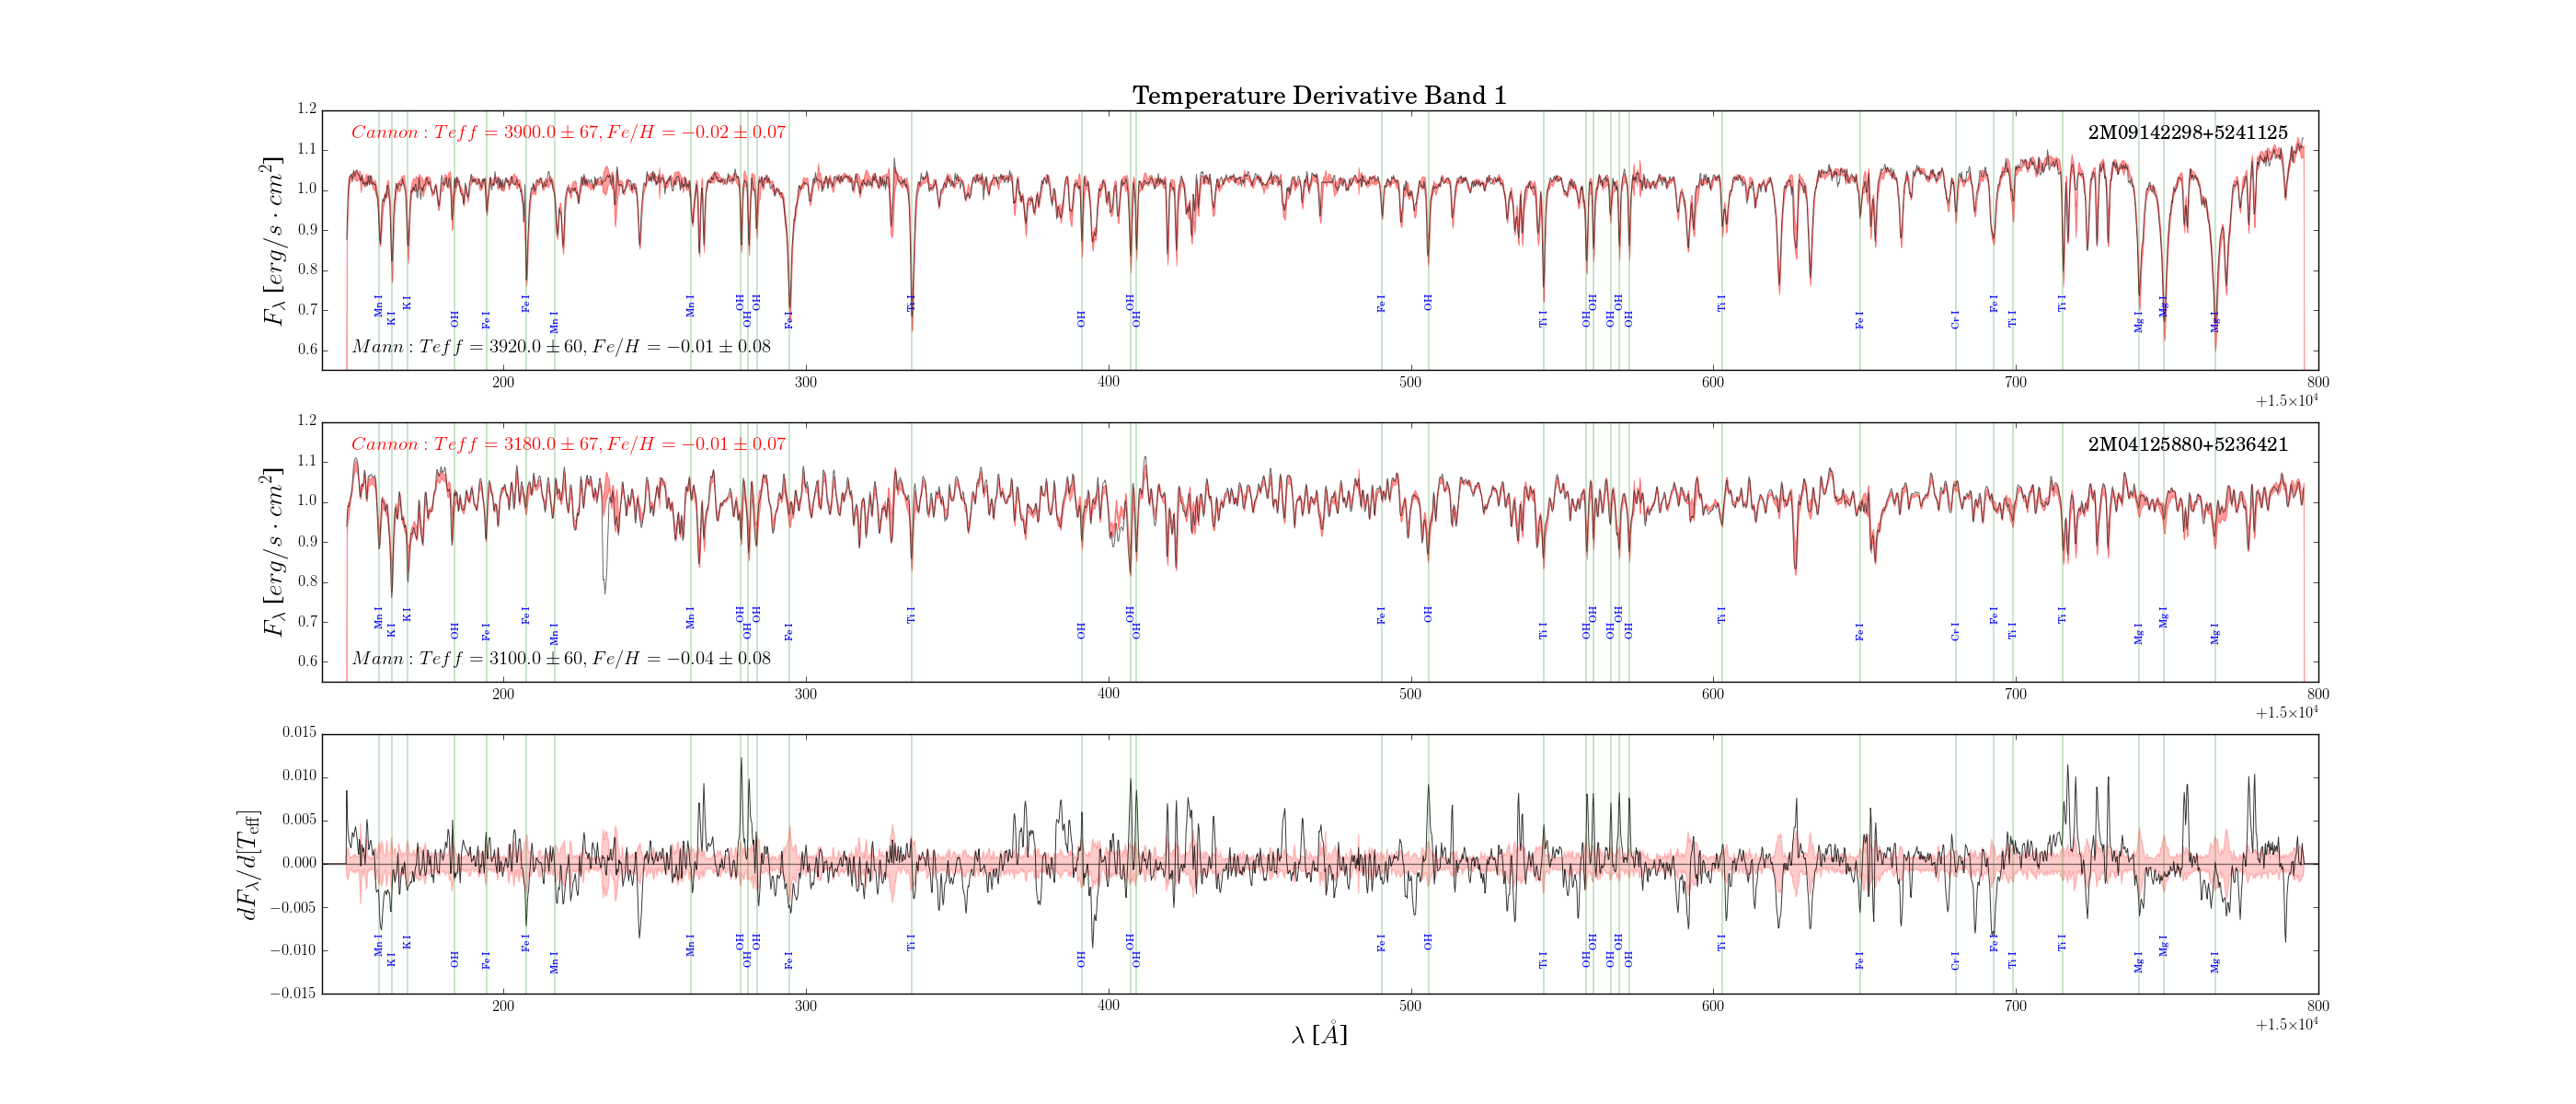
\includegraphics[width=16cm]{figures/demo_derivatives_teff1.png}
	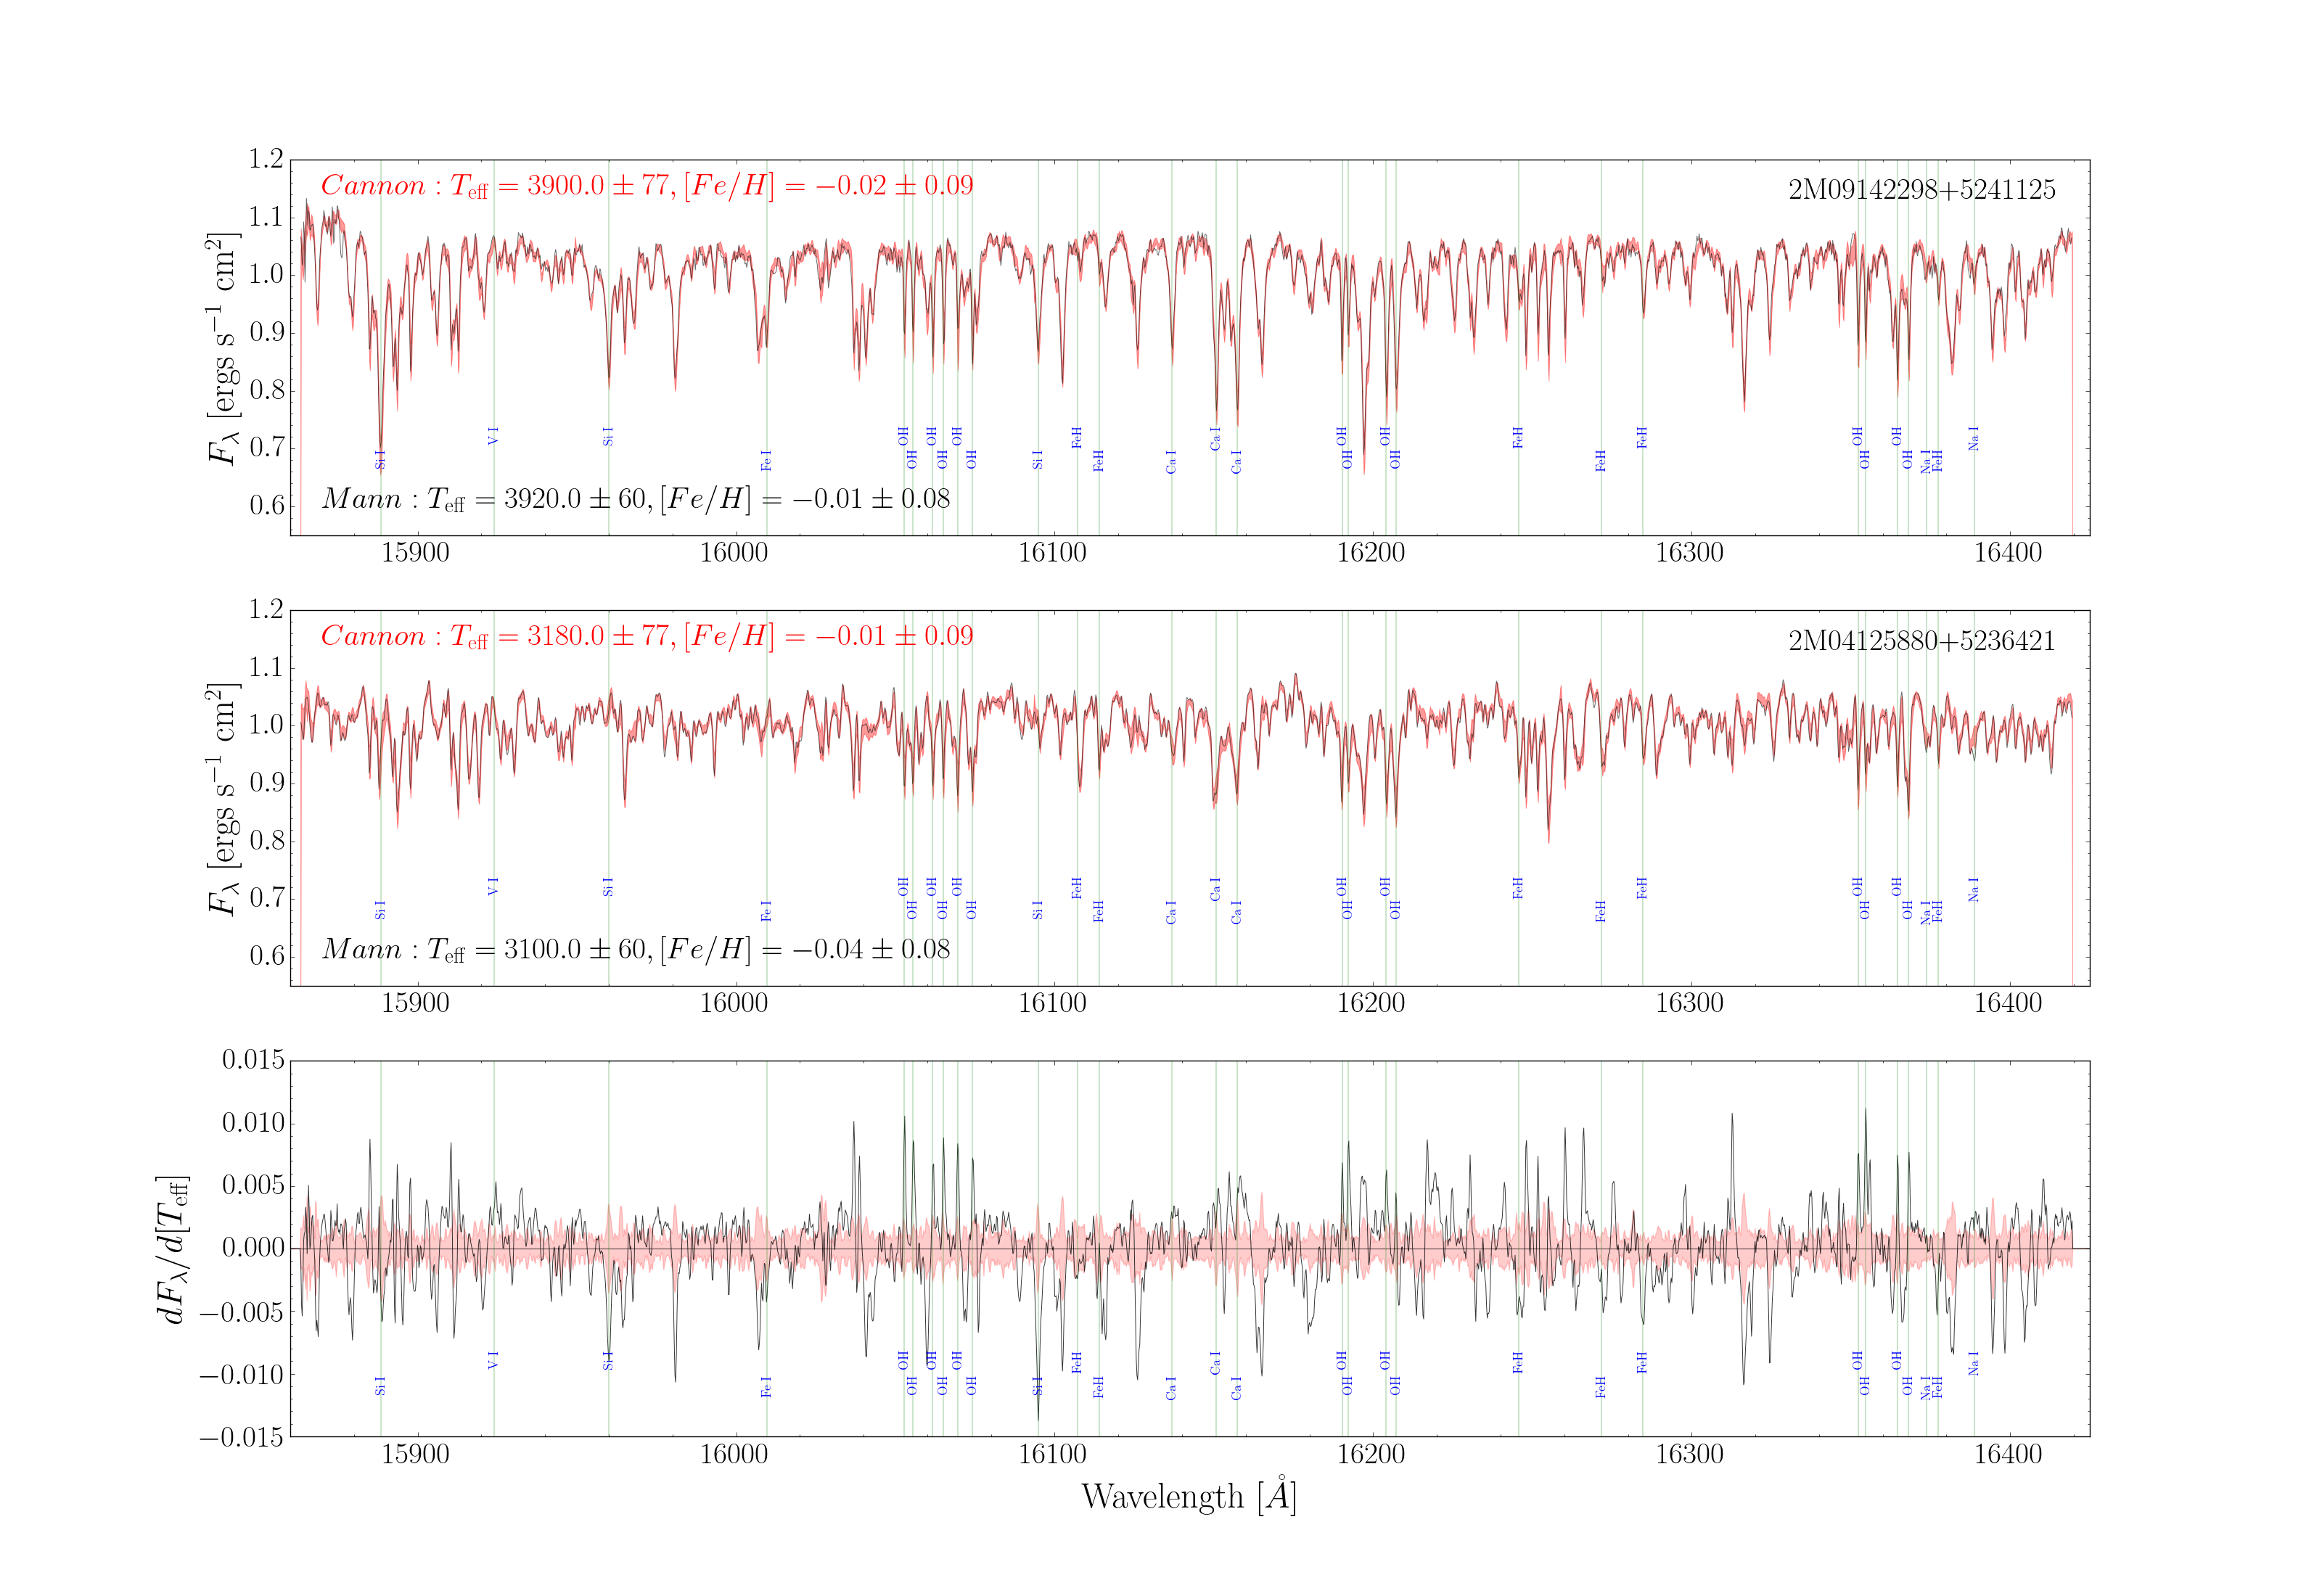
\includegraphics[width=16cm]{figures/demo_derivatives_teff2.png}
	\end{center}
\end{figure*}

\begin{figure*}[ht]
	\begin{center}
	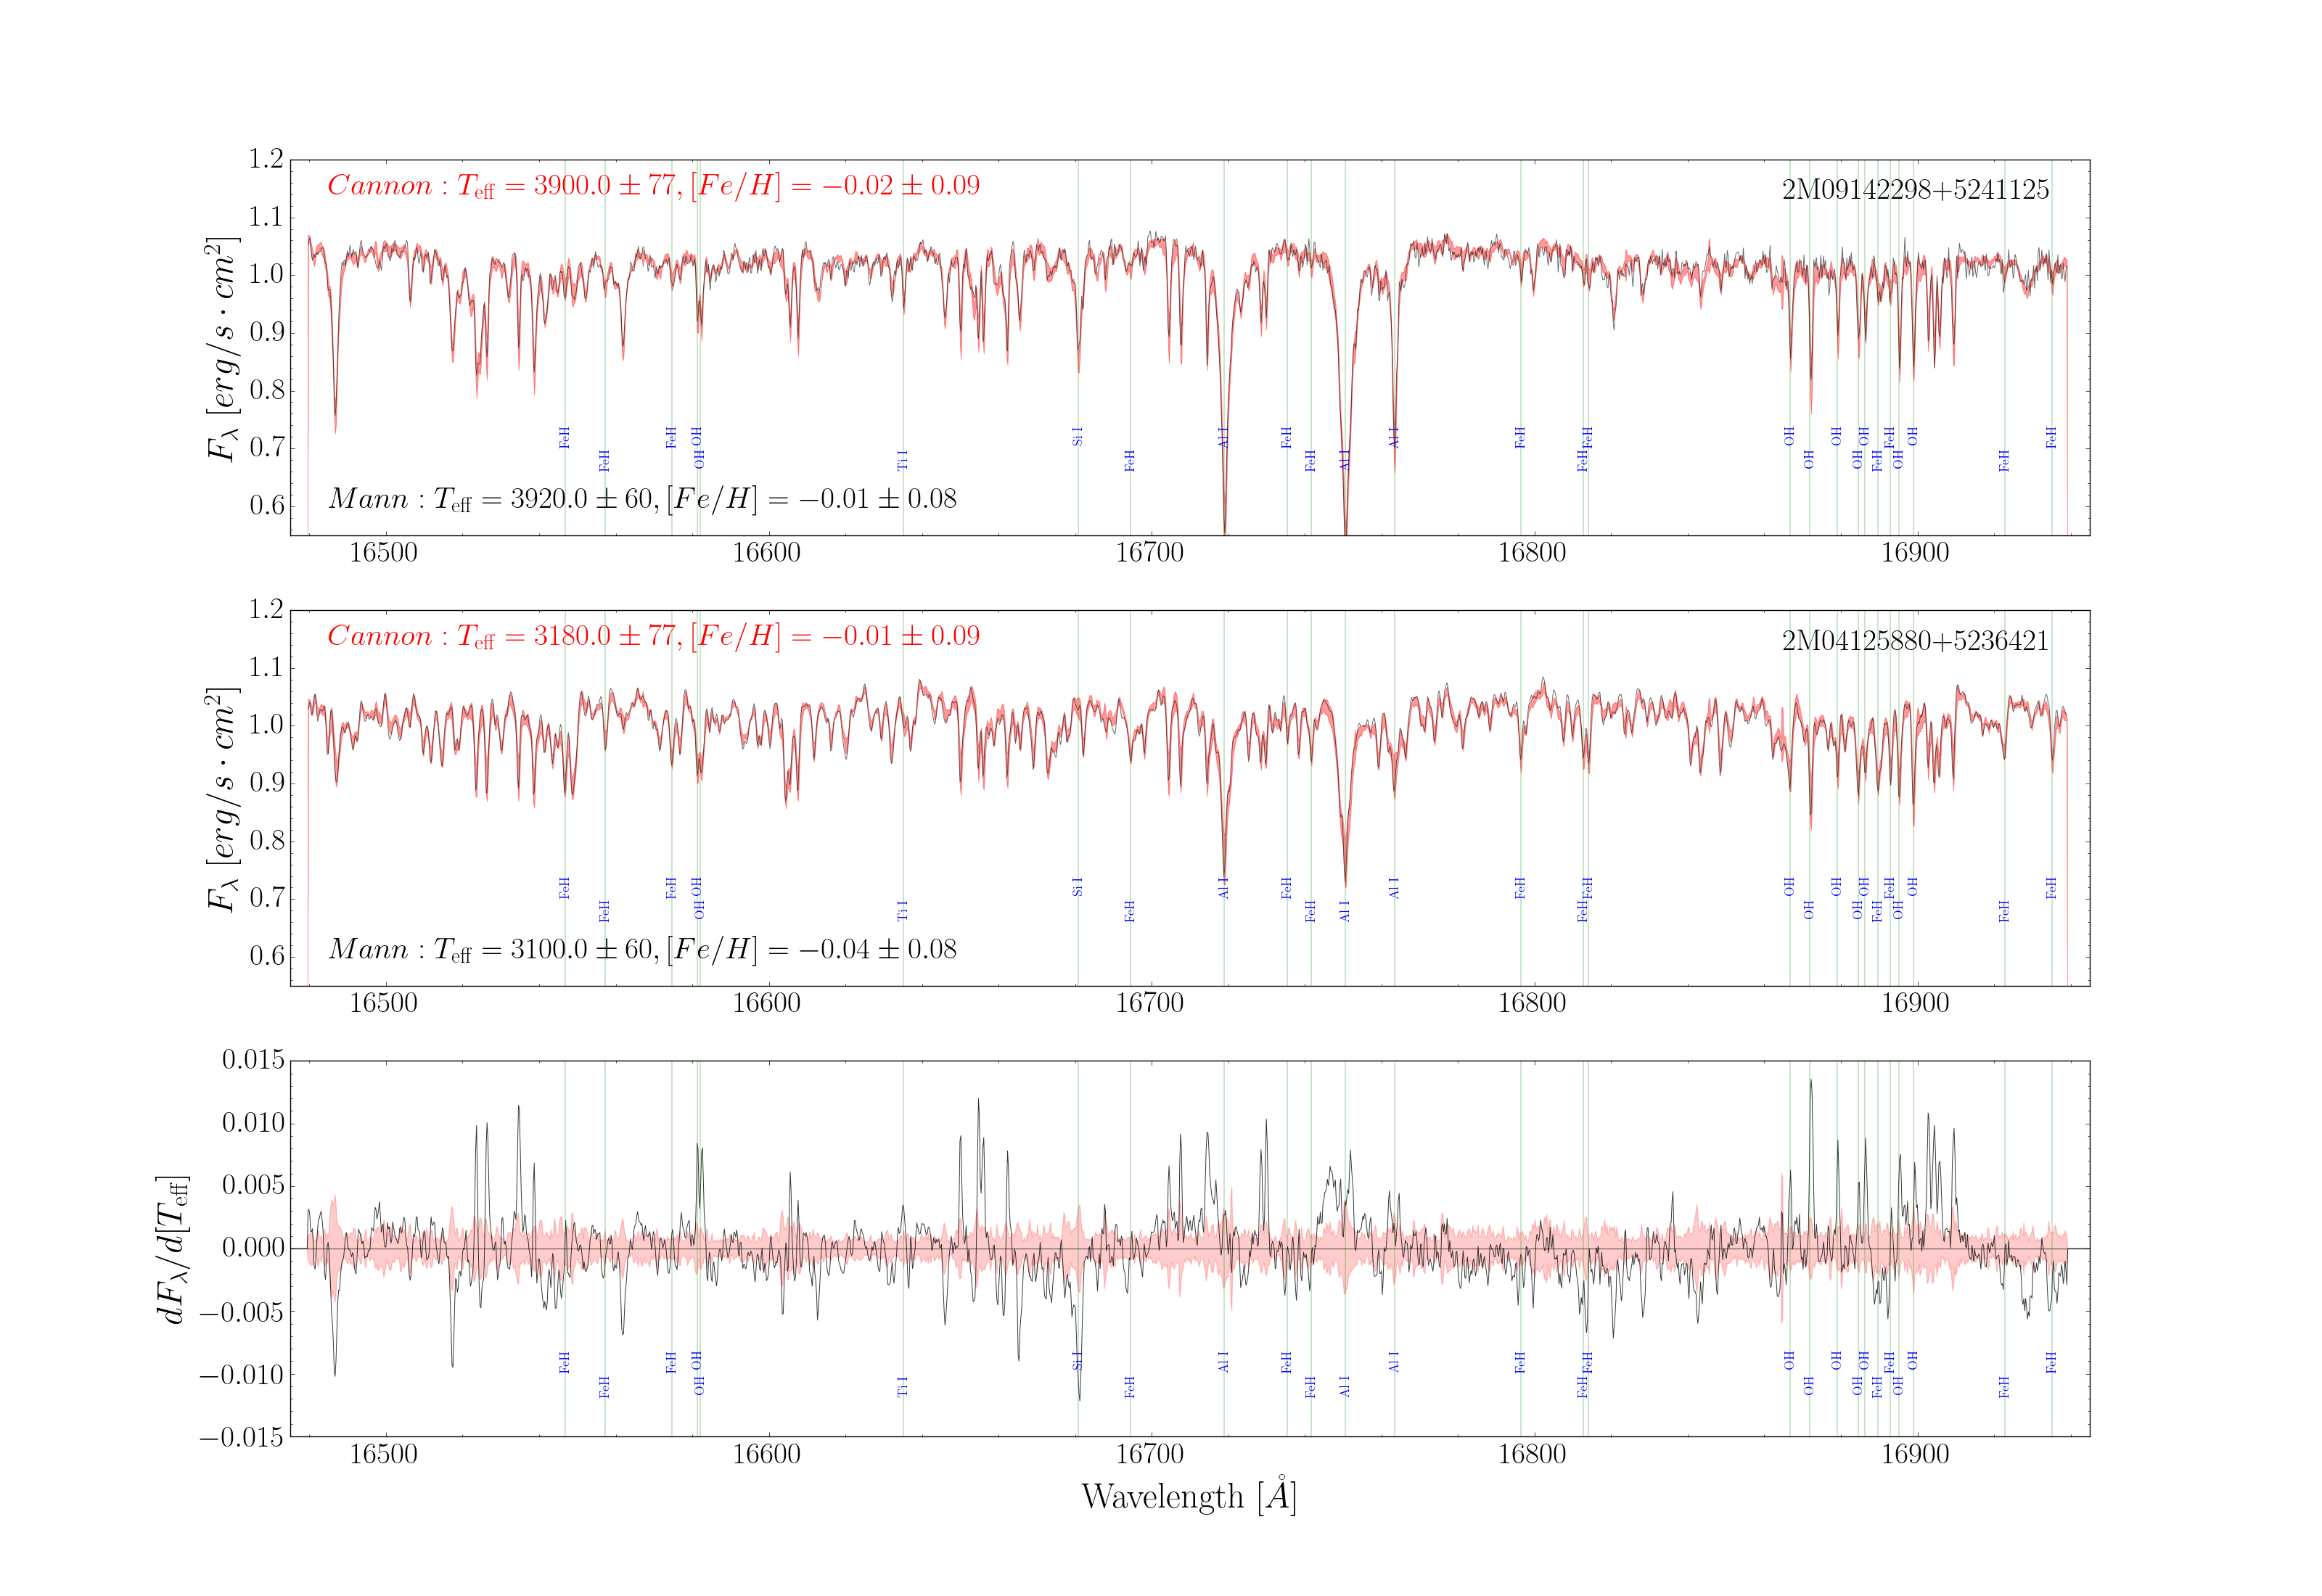
\includegraphics[width=16cm]{figures/demo_derivatives_teff3.png}
	\end{center}
	\caption{\textit{Top two panels of each plot:} Mann-trained model for varying temperatures, and similar metallcities. \textit{Third panel of each plot:} Derivative of \thecannon\ model with respect to temperature, taken at the median training temperature, T$_{\rm eff}=3463$K; error estimate computed using a jackknife statistic at each pixel is marked in red, making it possible to distinguish which features vary significantly with change in spectral type, and which are likely due to noise.}\label{fig:demo_teff}
\end{figure*}

%---------------------------
\begin{figure*}[ht]
	\begin{center}
	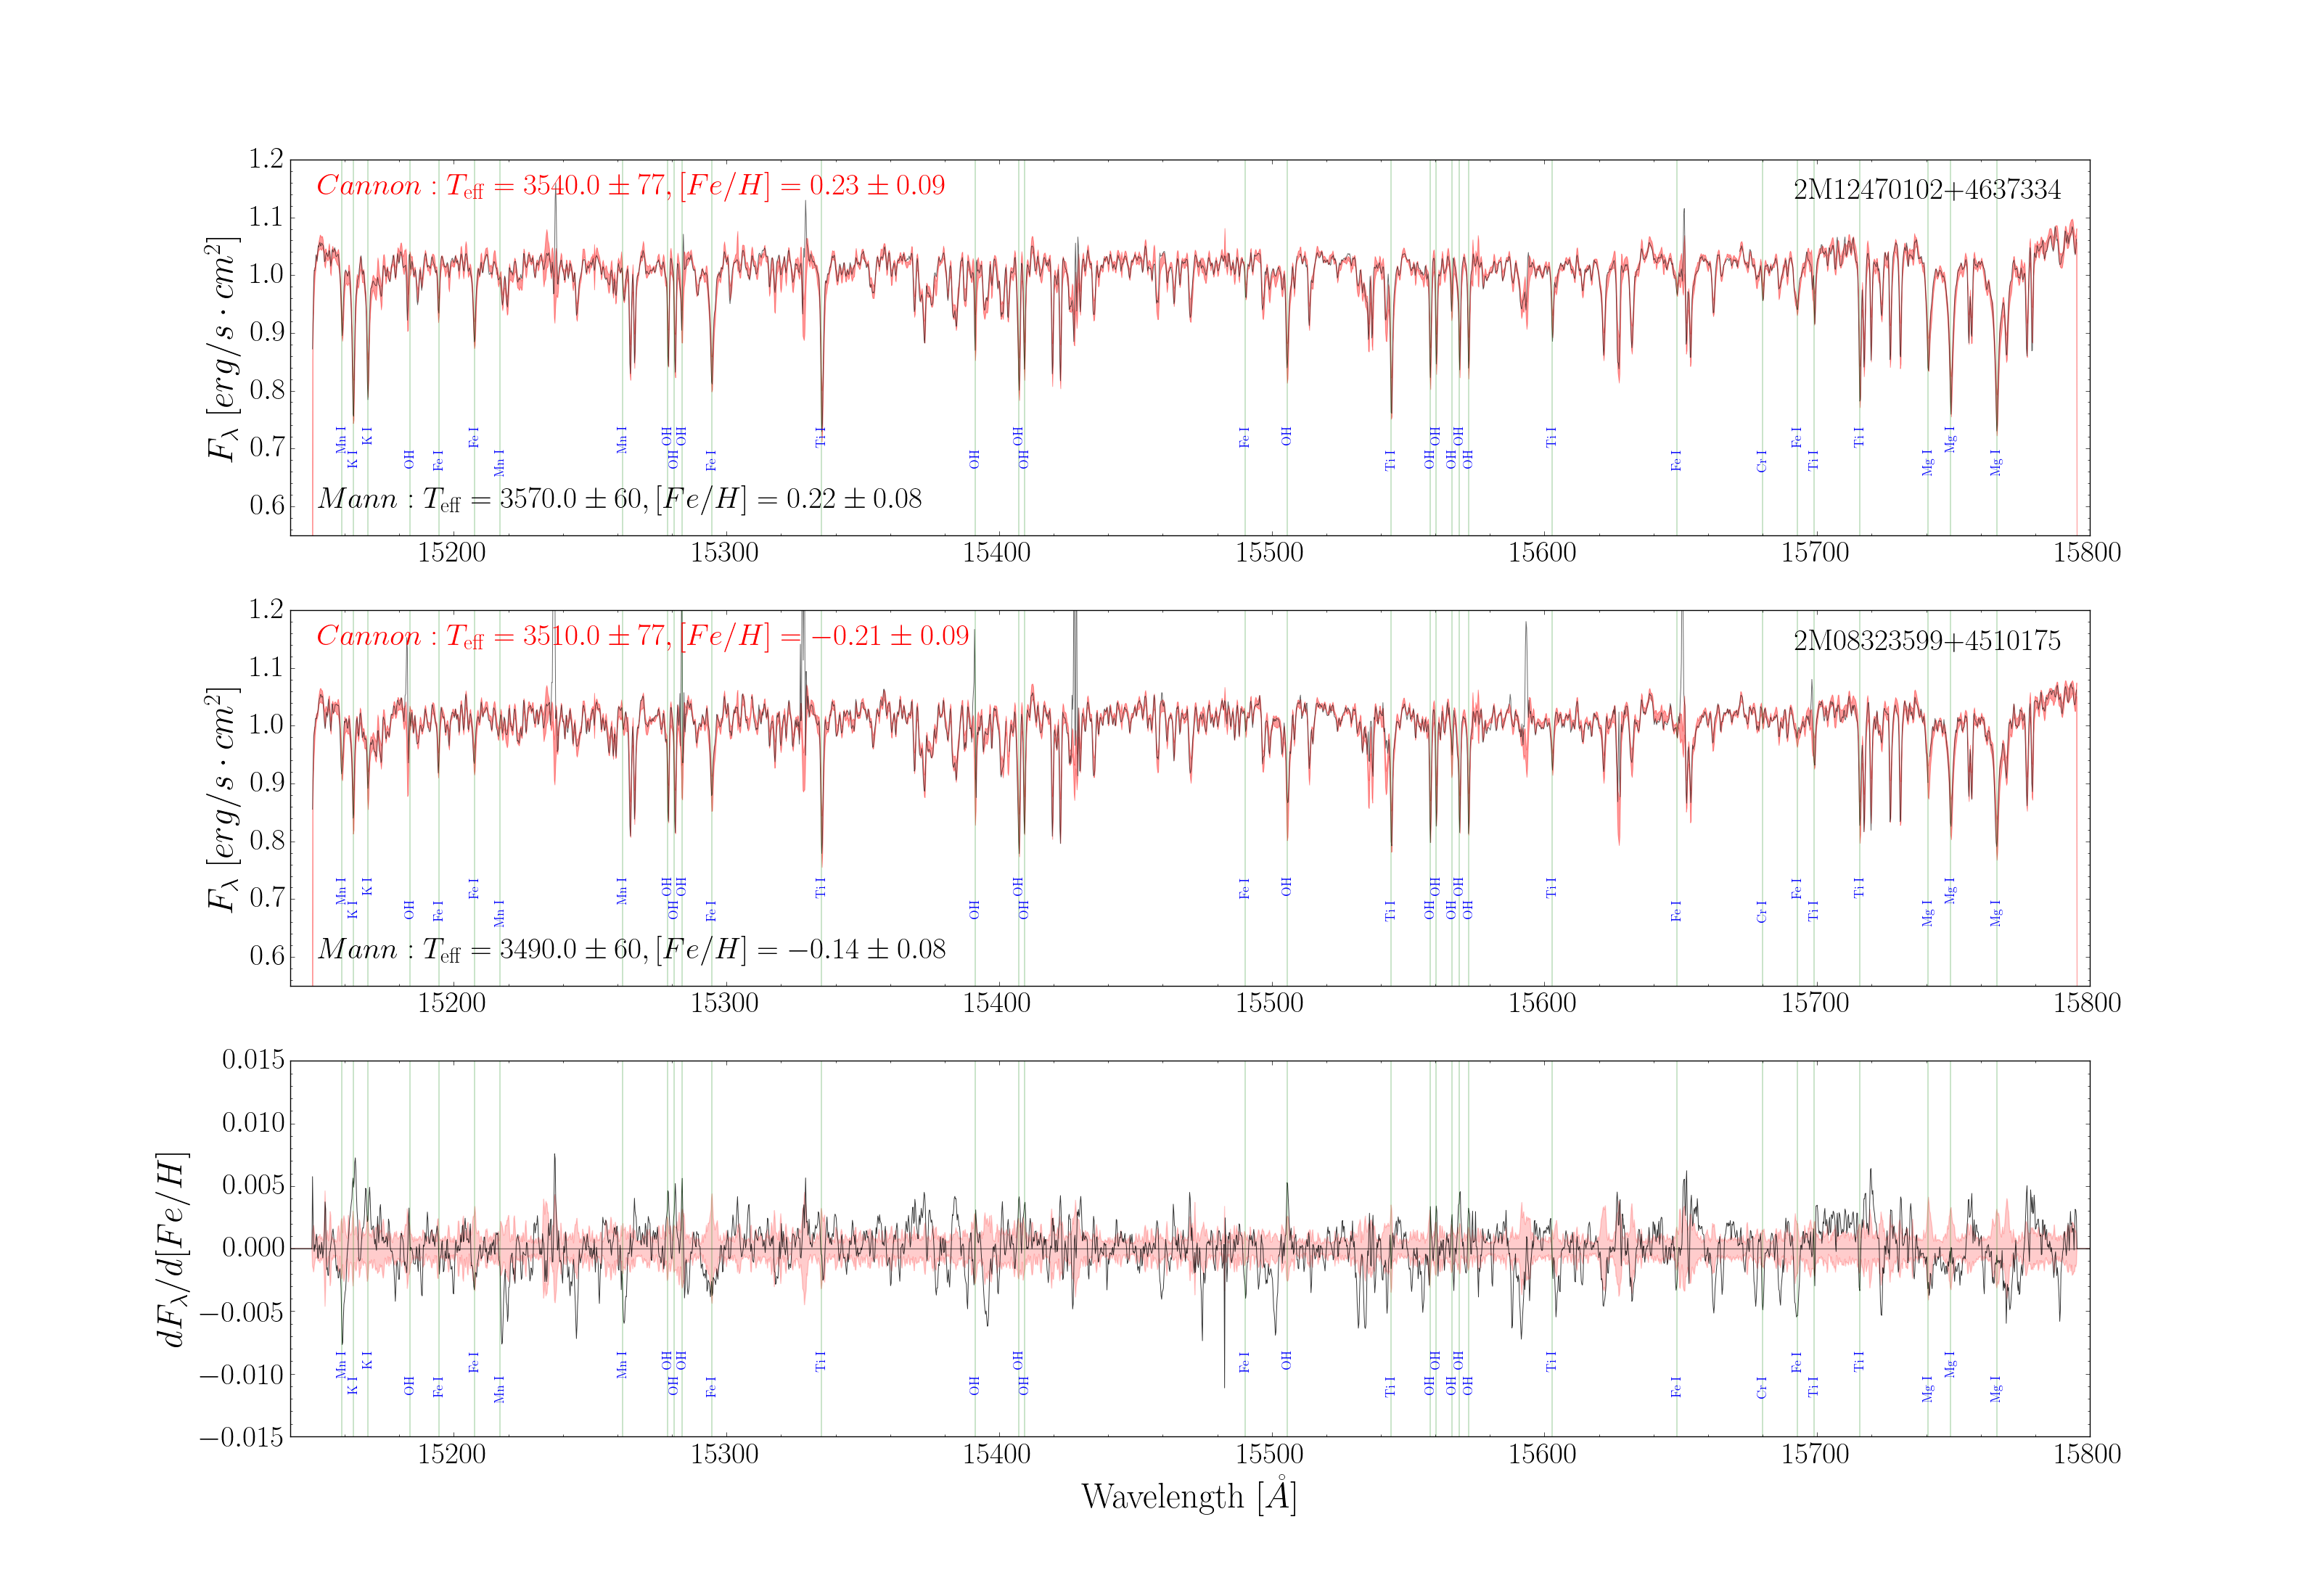
\includegraphics[width=16cm]{figures/demo_derivatives_feh1.png}
	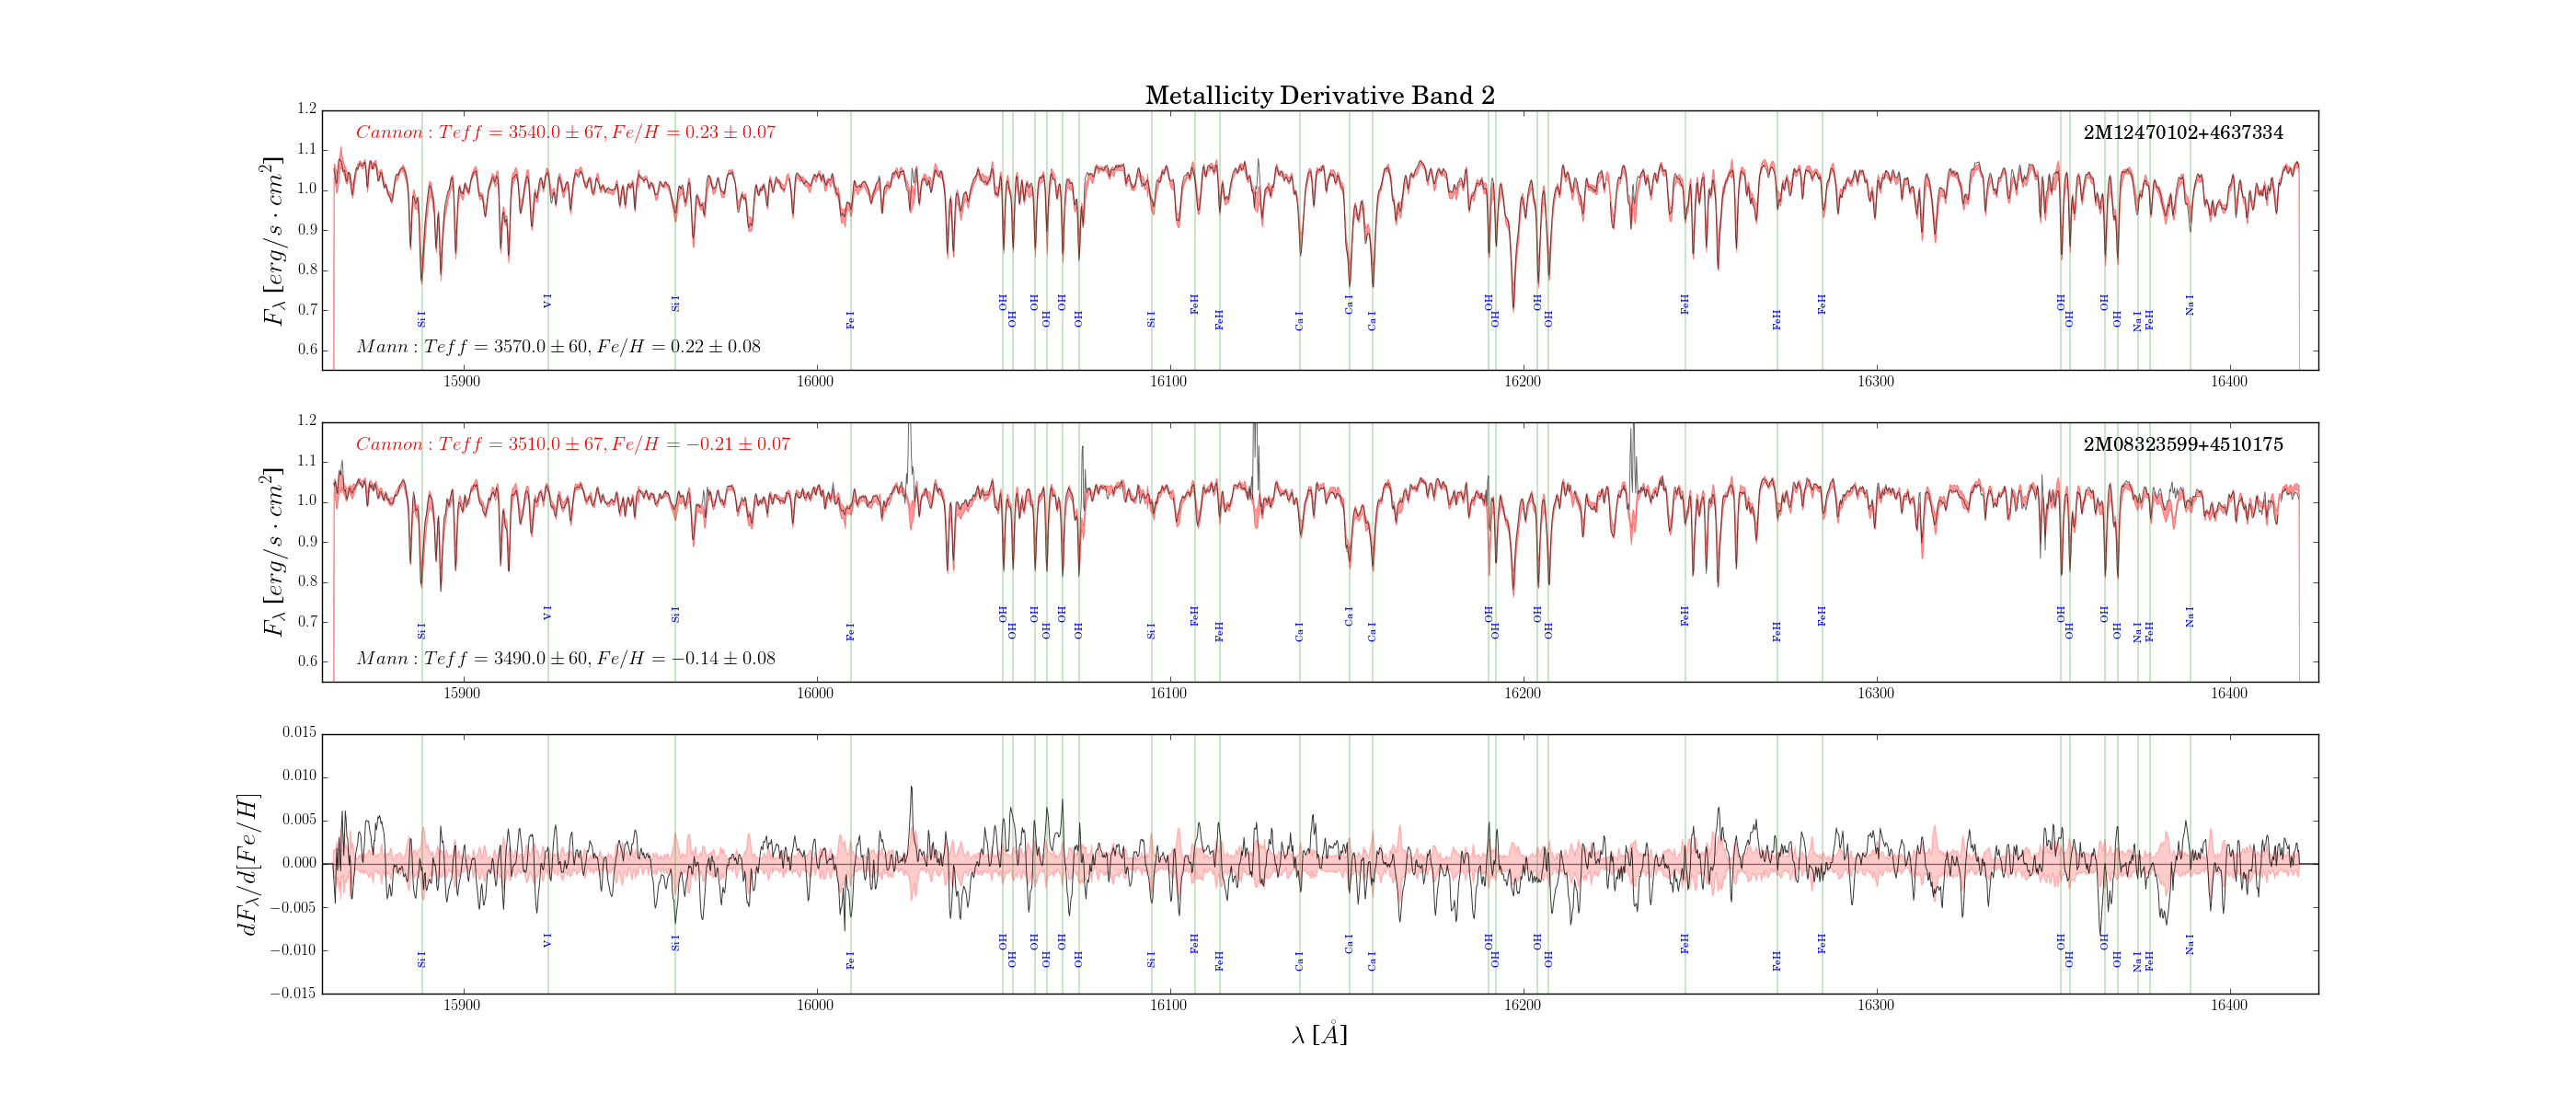
\includegraphics[width=16cm]{figures/demo_derivatives_feh2.png}
	\end{center}
\end{figure*}

\begin{figure*}[ht]
	\begin{center}
	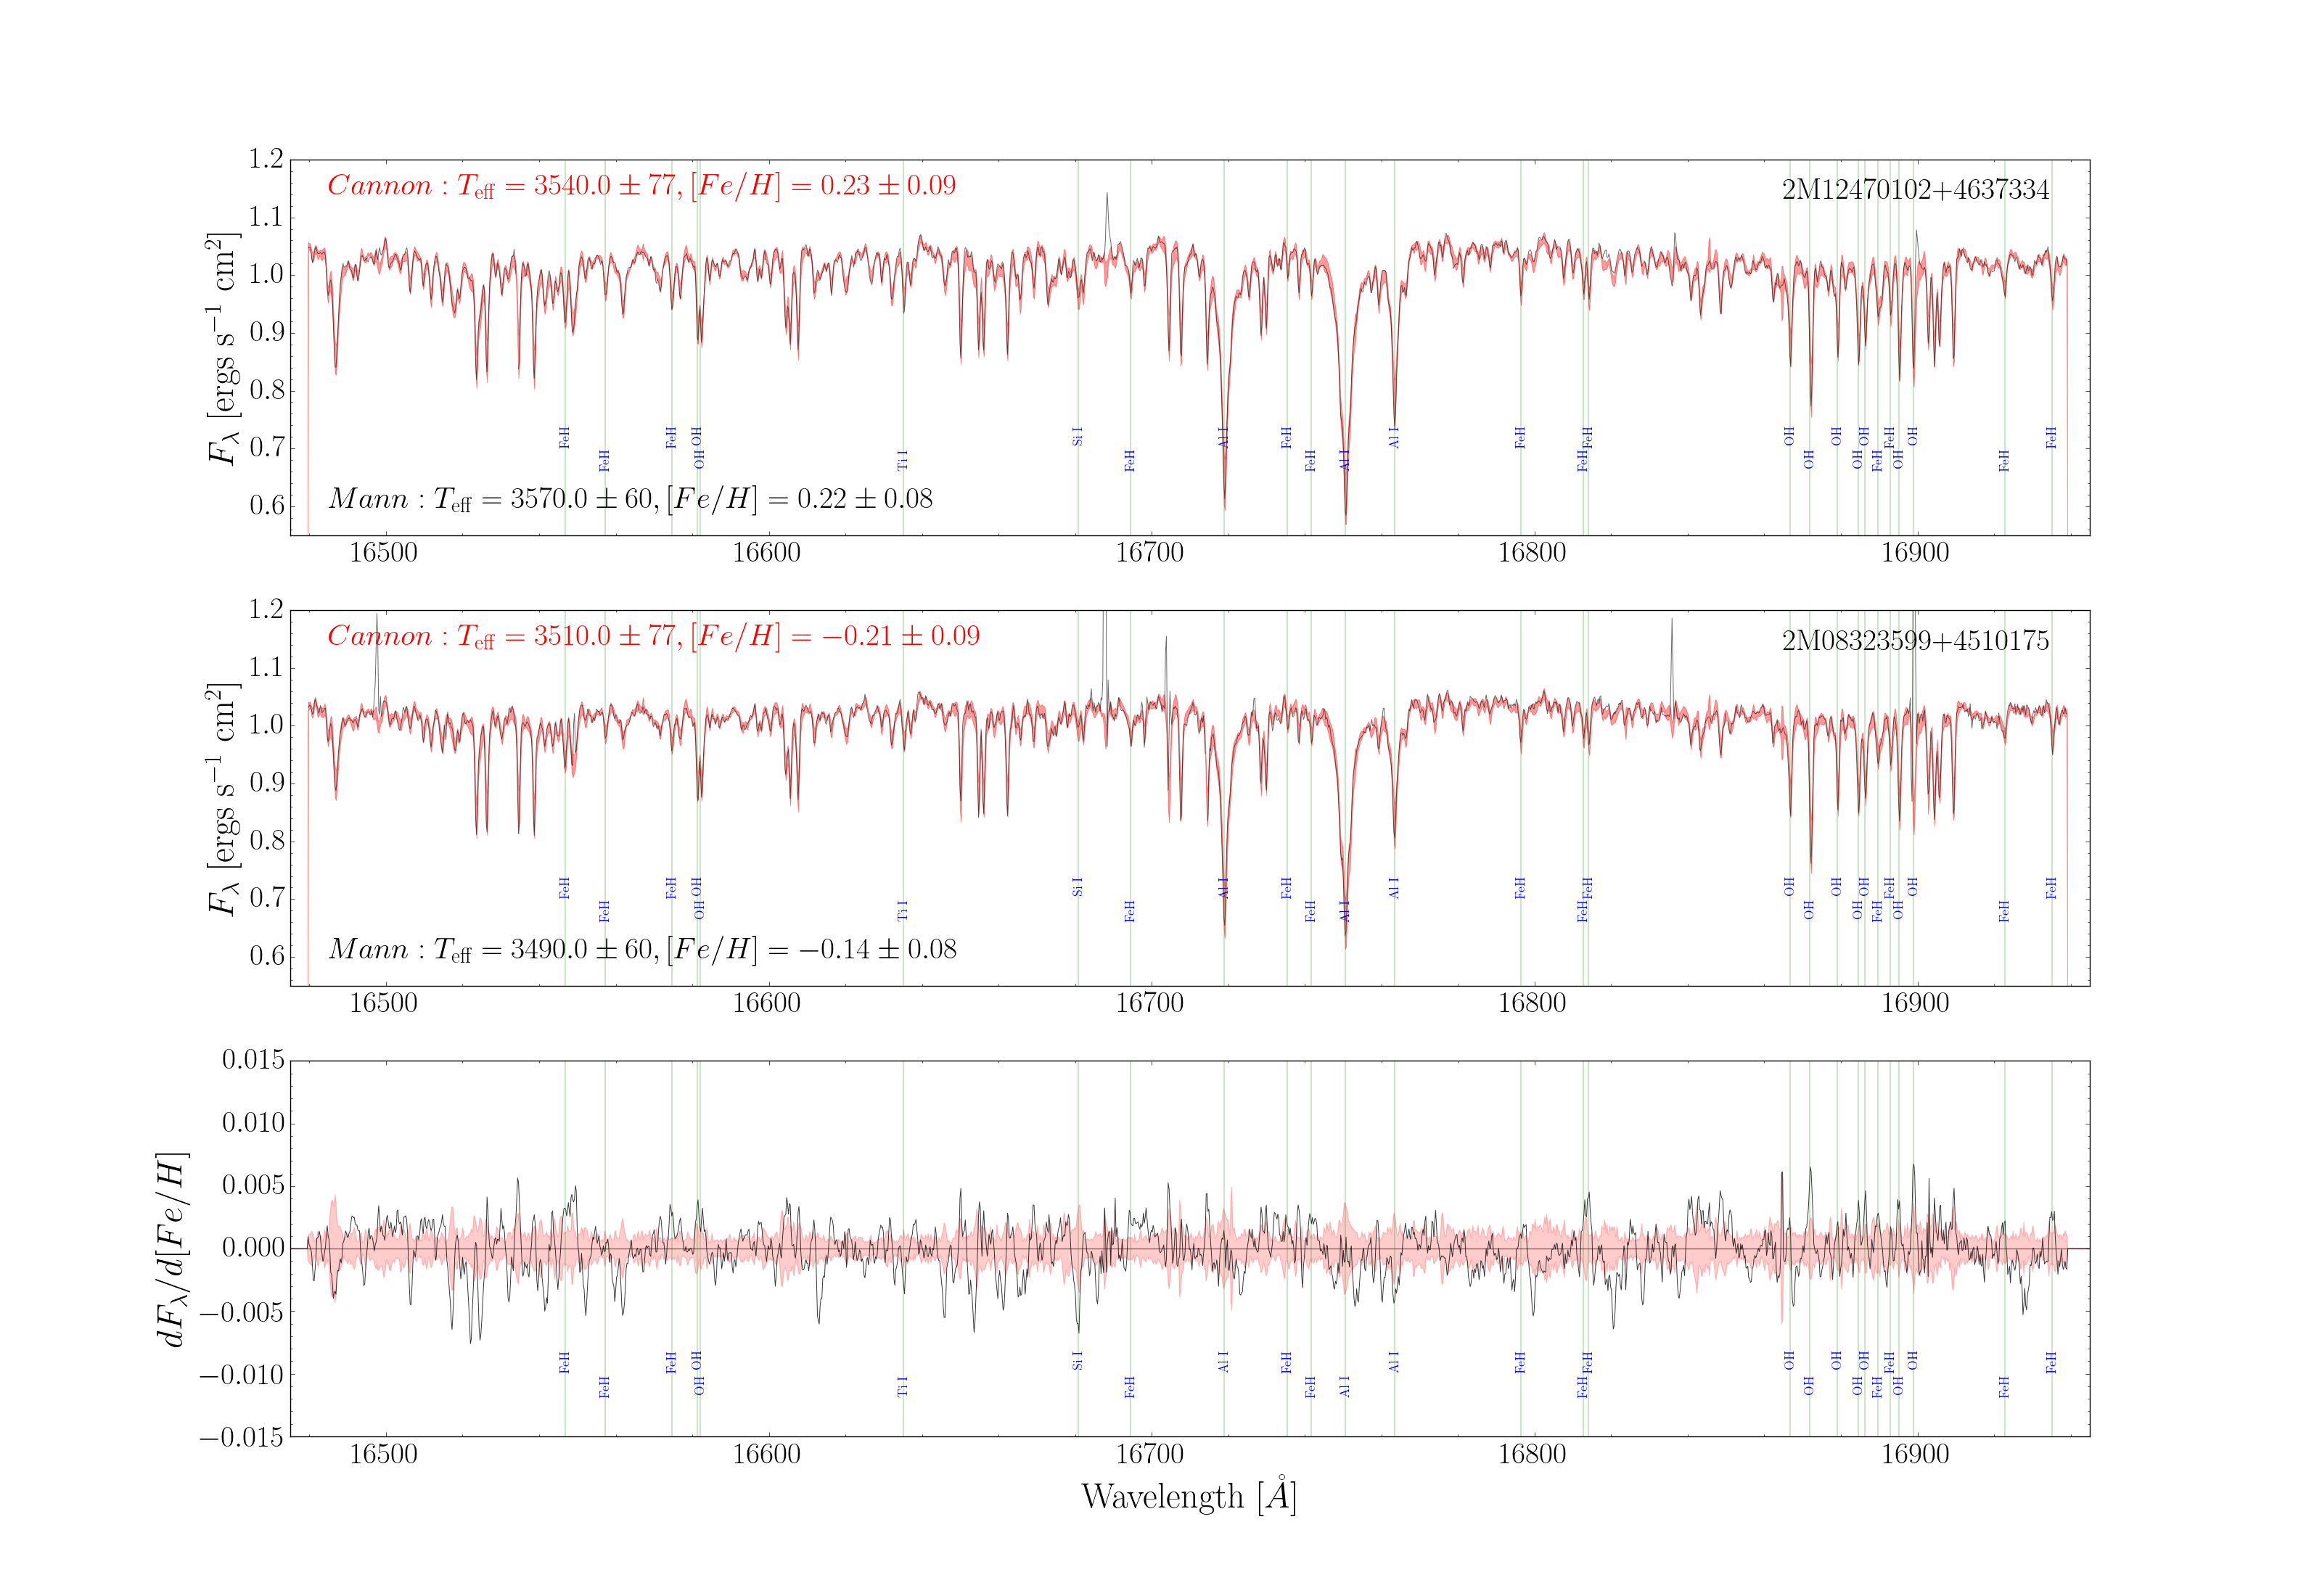
\includegraphics[width=16cm]{figures/demo_derivatives_feh3.png}
	\end{center}
	\caption{\textit{Top two panels of each plot:} Mann-trained model for varying metallicities and similar temperatures. \textit{Third panel:} Derivative of \thecannon\ model with respect to metallicity, taken at the median training metallicity, $\feh=-0.03$\,dex; jackknife computed error at each pixel is shown in red.} \label{fig:demo_feh}
\end{figure*}

%---------------------------
\begin{figure*}[ht]
	\begin{center}
	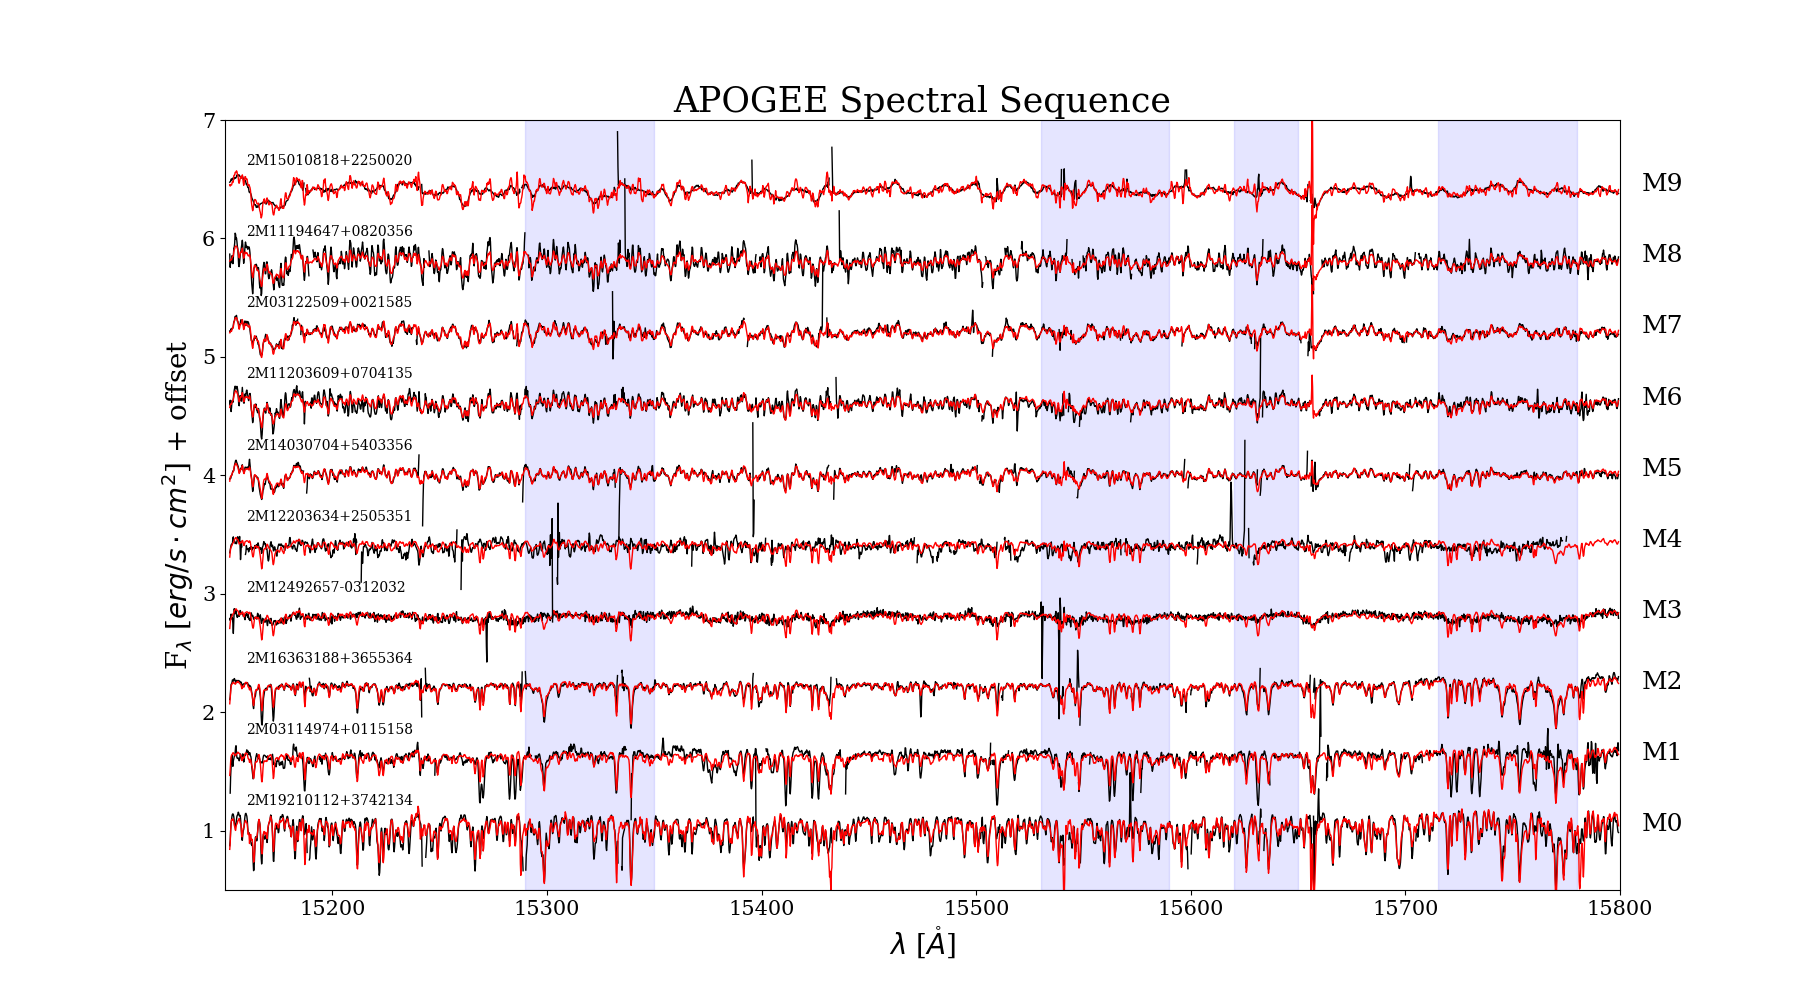
\includegraphics[width=12cm]{figures/Spectral_Sequence_1.png}
	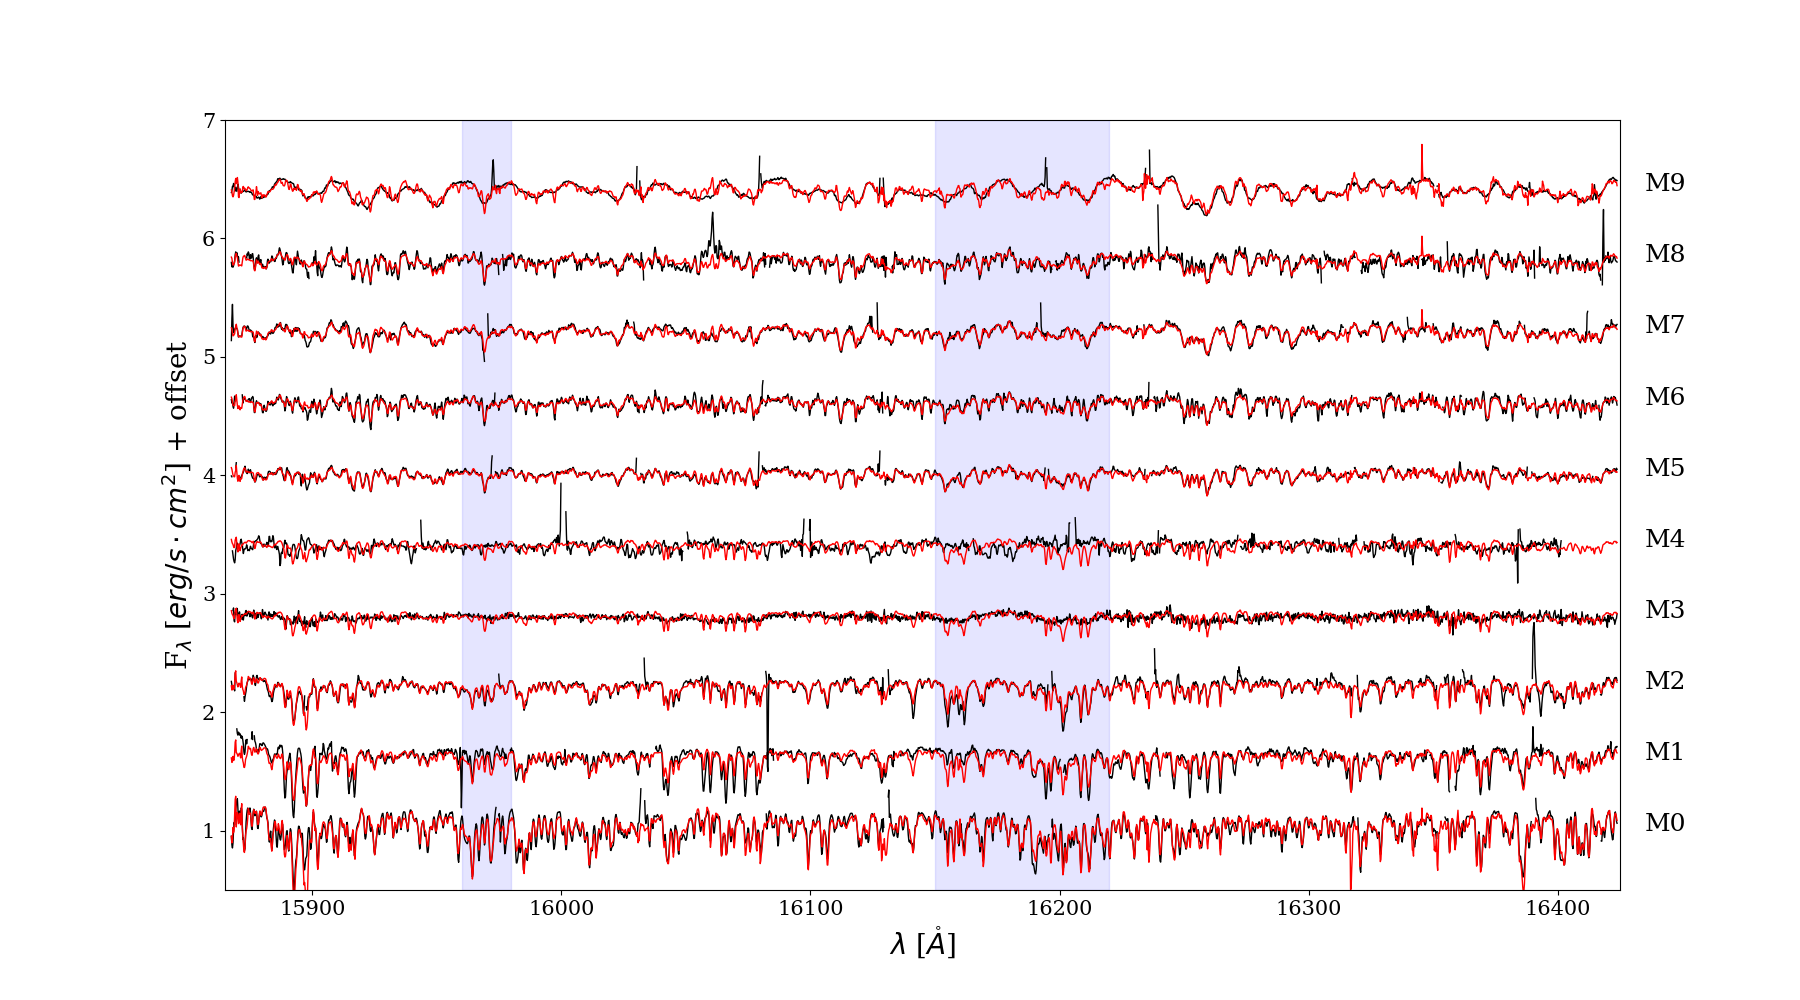
\includegraphics[width=12cm]{figures/Spectral_Sequence_2.png}
	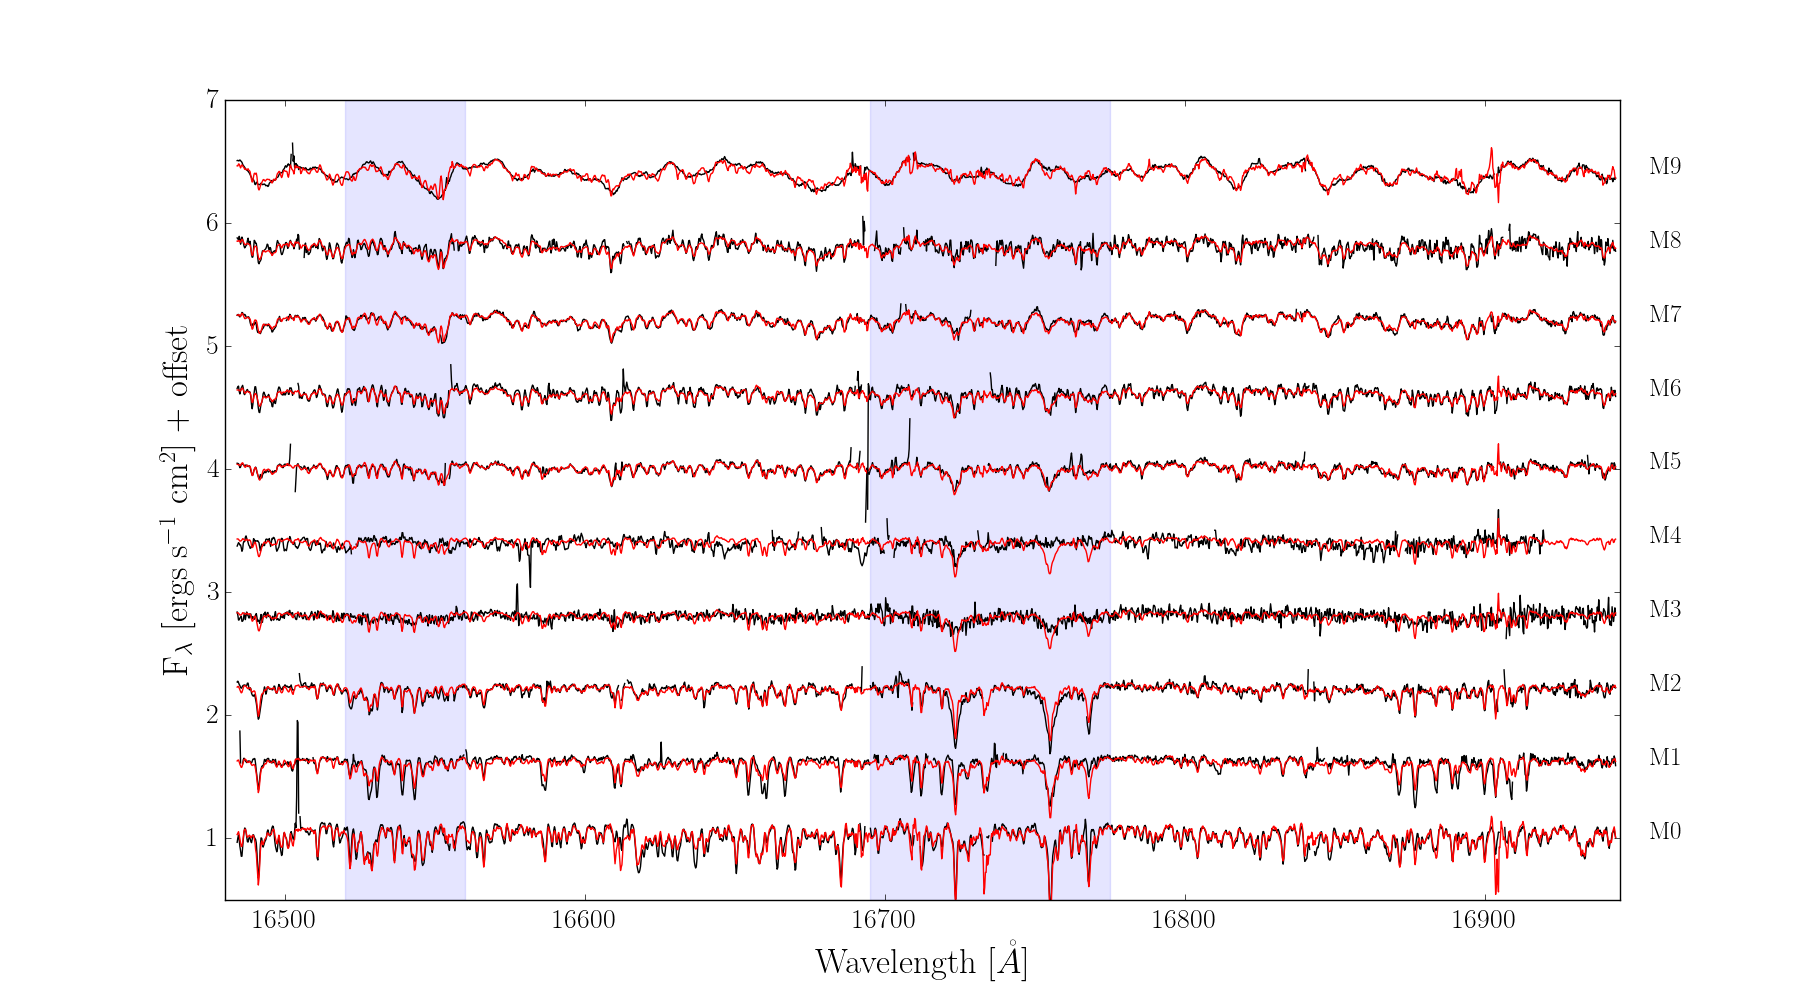
\includegraphics[width=12cm]{figures/Spectral_Sequence_3.png}
	\end{center}
	\caption{Spectral sequence of dwarfs in training set M0-M9; separate plots show three detector chips of \apogee\ spectrum (black), the best fit Cannon trained model (red) with highlighted spectral type sensitive regions identified in \citealt{Desphande:2013}.} \label{fig:sp_sequence}
\end{figure*}

%---------------------------
\begin{figure*}[ht]
	\begin{center}
	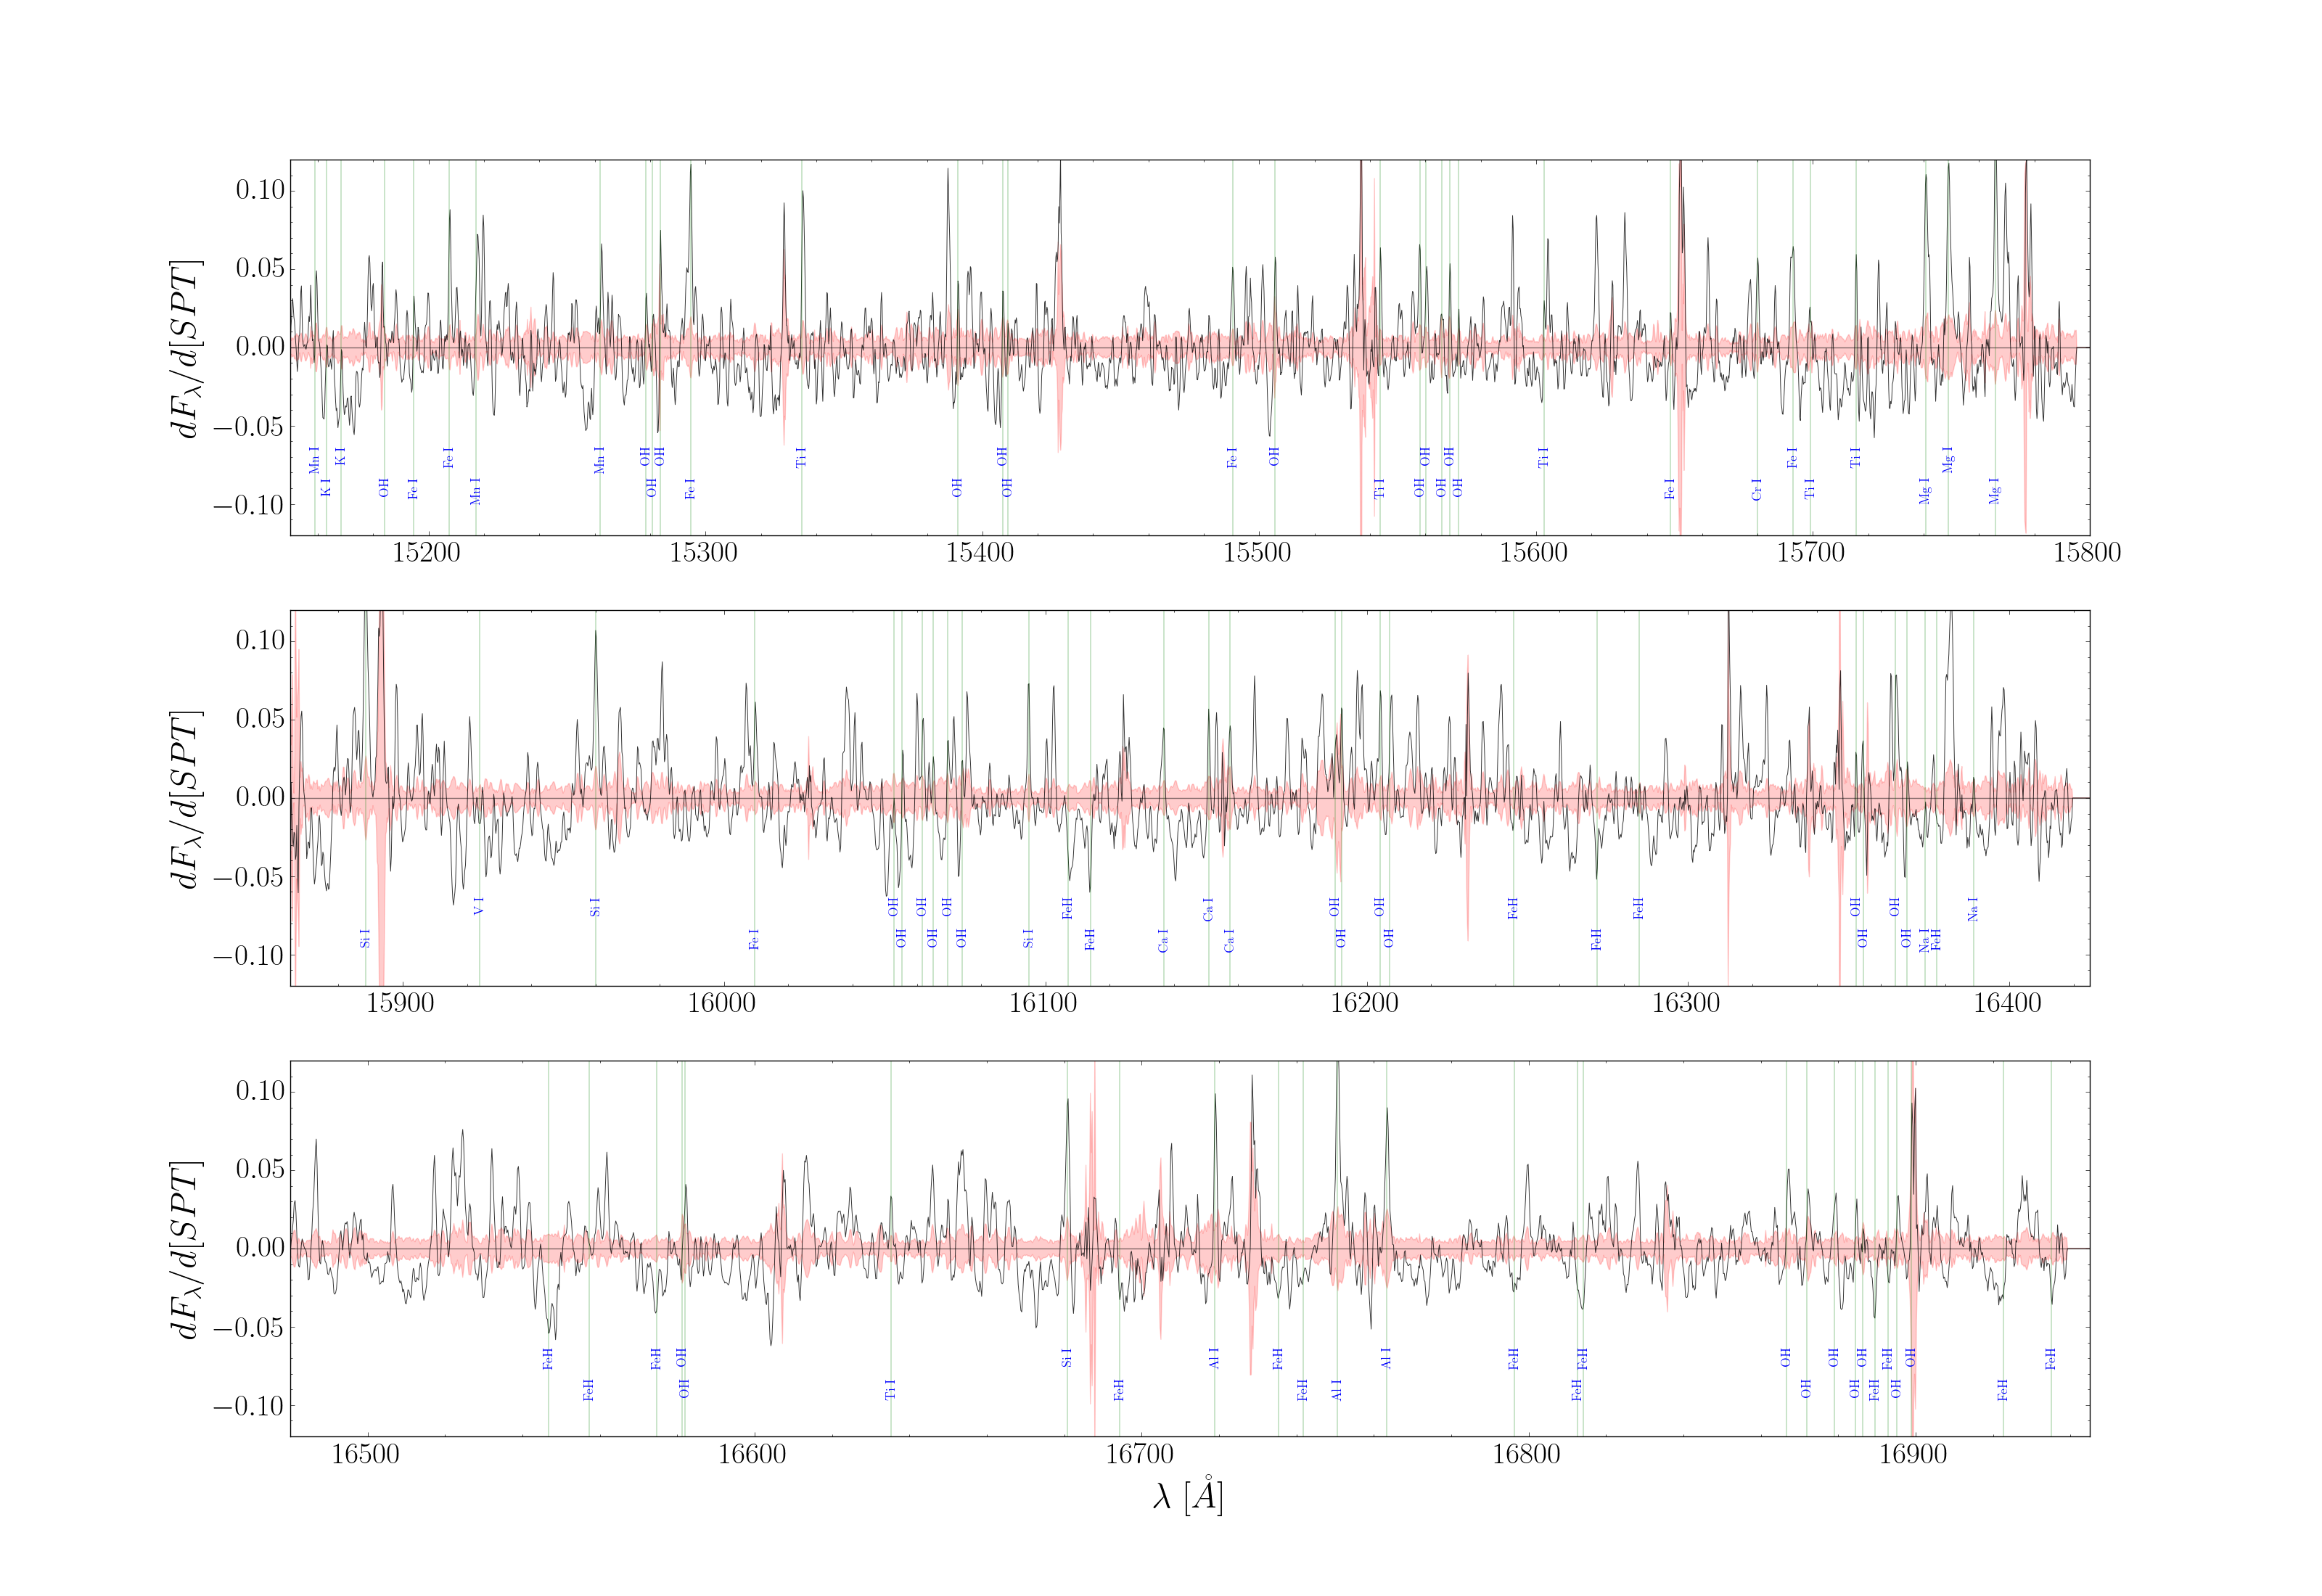
\includegraphics[width=16cm]{figures/derivative_jackknife_spt.png}
	\end{center}
	\caption{Derivative plots for spectral type model taken at the median training spectral type, SPT$=3$; jackknife computed error at each pixel is shown in red.} \label{fig:west_derivative}
\end{figure*}

\begin{figure*}[ht]
	\plotone{figures/cannon_chi_dist.png}
	\caption{\textit{Left:} the distribution of fits for the training sample and known samples of pre-MS stars (\citealt{Cottaar:2014}) and binary sources (\citealt{ElBadry:2018}; \citealt{Skinner:2018}); \textit{right:} the distribution of $\chi^2$ fits for all 14,827 sources in the \apogee --\gaia\ cross match, with color cuts $1<G_{BP}-G_{RP}<6$ and $7.5<M_{G}<20$ and $\varpi>0$. We apply a quality cut of $\chi^2 < 100,000$ to the test sample for those sources we report as ``safe''. \label{fig:chi_dist}}
\end{figure*}

\begin{figure*}[ht]
	\plotone{figures/cmd_selection.png}
	\caption{\gaia\ and \zmass\ color-magnitude cuts for 12,037 sources with $\chi^2<100,000$. Over plotted with orange triangles are the 67 out of 87 training sample sources which have parallaxes measured by \gaia. \label{fig:cmd_selection}}
\end{figure*}

\begin{figure*}[ht]
	\plottwo{figures/cmd_teff_full.png}{figures/cmd_teff_safe.png}
	\plottwo{figures/cmd_feh_full.png}{figures/cmd_feh_safe.png}
	\plottwo{figures/cmd_spt_full.png}{figures/cmd_spt_safe.png}
	\caption{Full sample of 14,827 M dwarfs colored by \cannon\ labels before selection (left) and final sample selection of 10,311 M dwarfs after applying selection criteria described in Section \ref{subsec:test_selection} (right), to reduce contamination from sources with that are not similar to the training sample (not single, main-sequence M stars, such as pre-main sequence, binaries, and K dwarfs). Overplotted with orange triangles are the M15 and W11 training samples, for their respective \cannon\ test labels. Temperature gradient increases with decreasing color, spectral subtype increases with increasing color, and metallicity gradient increases perpendicularly up from the main sequence branch as expected. Deviations from these gradients seen at the upper slice of the main sequence is likely remaining contamination from the binary sequence. \label{fig:safe_selection}}
\end{figure*}

\begin{figure*}[ht]
	\plotone{figures/spt_vs_teff_vs_feh.png}
	\caption{West-trained spectral types vs. Mann-trained metallcities and temperatures. For each integer spectral type bin the mean temperatures and metallicities are shown as red error boxes. \label{fig:west_vs_mann}}
\end{figure*}

\begin{figure*}[ht]
	\plotone{figures/aspcap_cannon_label_hist.png}
	\caption{Distribution of temperatures and metallicities for 10,311 sources from \thecannon\ compared to the \aspcap\ pipeline. Note that \cannon\ temperatures only span $2850<T_{\rm eff}<4150$ and $-0.5<\feh<0.5$\,dex because we have imposed cutoffs for stars that fall outside of the training sample range, however for the same 10,311 stars \aspcap\ predicts temperatures with slightly higher temperatures and metallicities. \label{fig:aspcap_cannon_label_hist}} 
\end{figure*}

%---------------------------
\begin{figure*}[ht]
	\plotone{figures/aspcap_cannon_validation.png}
	\caption{\cannon\ (right column) and \aspcap\ (left column) temperatures as compared to temperatures estimated color-temperature relations from three different literature sources for a subsample of 6,257 sources with $V,J,K$ colors. Shown are \cannon\ and \aspcap\ temperatures (x-axis) compared to temperatures estimated from the \citealt{Mann:2015} $V-J$ and $\feh$ dependent relation (top), \citealt{Casagrande:2008} $V-K$ relation (middle), and the \citealt{Boyajian:2012} relation $V-K$ and $\feh$ (bottom).  \label{fig:teff_comparisons}}
\end{figure*}

%---------------------------
\begin{figure*}[ht]
	\plotone{figures/isochrone_cmd.png}
	\caption{Comparison of \cannon\ $\feh$ as compared to metallicity predicted by PARSEC isochrone tracks \citealt{Bressan:2012} in \gaia\ color-magnitude space. The four panels show five metallicity tracks (ranging $-0.5<$[M/H]$<0.5$) over varying ages (1, 3, 5, and 7 Gyr). \label{fig:isochrone_cmd}}
\end{figure*}

\begin{figure*}[ht]
	\plotone{figures/mann_radii.png}
	\caption{Comparison of radii estimated from M15 relations: on the x-axis radii are derived from  K magnitudes and \cannon\ $\feh$, on the y-axis radii are derived from \cannon\ $\teff$ and $\feh$. \label{fig:radii}}
\end{figure*}

%%==========================================================================================
%% Tables

% \newpage 

\begin{longrotatetable}
\begin{deluxetable*}{ccc|ccc|ccc|c}
\tablecaption{Cannon results for Temperature/Metallicity model; see online journal for full table. \label{table:mann_results}}
\tabletypesize{\scriptsize}
\tablehead{
\multicolumn{3}{c}{\underline{Designation}} & \multicolumn{3}{c}{\underline{Temperature (K)}} & \multicolumn{3}{c}{\underline{Metallicity (dex)}} & \multicolumn{1}{c}{\underline{Model Fit}} \\
	  \colhead{2MASS ID} & \colhead{RA}   & \colhead{DEC}
    & \colhead{Training} & \colhead{Test} & \colhead{LOOCV}
    & \colhead{Training} & \colhead{Test} & \colhead{LOOCV} 
    & \colhead{Test $\chi^2$} 
} 
	\startdata
	2M00182256+4401222 & 4.59542   & 44.02278  & 3603        & 3538       & 3525        & -0.3       & -0.28     & -0.26      & 15304   \\
	2M00182549+4401376 & 4.60779   & 44.02734  & 3218        & 3528       & 3560        & -0.3       & -0.29     & -0.29      & 21273   \\
	2M00285391+5022330 & 7.22488   & 50.37588  & 3207        & 3190       & 3192        & 0.11       & 0.04      & 0.01       & 31790   \\
	2M00401001+0308050 & 10.04169  & 3.13473   & 3725        & 3777       & 3772        & 0.04       & 0.12      & 0.14       & 9830    \\
	2M00580115+3919111 & 14.50482  & 39.31977  & 3157        & 3100       & 3107        & -0.07      & -0.02     & 0.01       & 13337   \\
	2M01232542+1638384 & 20.8559   & 16.64401  & 3272        & 3225       & 3223        & 0.1        & 0.02      & -0.01      & 34797   \\
	2M02001278+1303112 & 30.05402  & 13.05196  & 3080        & 3059       & 3077        & -0.16      & -0.1      & -0.02      & 33210   \\
	2M02361535+0652191 & 39.06358  & 6.87167   & 3284        & 3241       & 3243        & -0.12      & -0.28     & -0.28      & 48445   \\
	2M03044335+6144097 & 46.18104  & 61.73583  & 3500        & 3466       & 3466        & -0.12      & -0.26     & -0.28      & 40739   \\
	2M03553688+5214291 & 58.90373  & 52.2414   & 3435        & 3386       & 3375        & -0.35      & -0.28     & -0.2       & 53870   \\
	2M04125880+5236421 & 63.24499  & 52.61165  & 3100        & 3183       & 3204        & -0.04      & -0.01     & 0.0        & 46007   \\
	2M04310001+3647548 & 67.75003  & 36.79855  & 3419        & 3371       & 3369        & 0.08       & 0.11      & 0.1        & 20602   \\
	2M05222053+3031097 & 80.58561  & 30.51933  & 3389        & 3423       & 3431        & 0.28       & 0.18      & 0.13       & 19072   \\
	2M05312734-0340356 & 82.86417  & -3.67722  & 3801        & 3814       & 3849        & 0.49       & 0.5       & 0.36       & 28209   \\
	2M05413073+5329239 & 85.37804  & 53.48987  & 3765        & 3751       & 3753        & 0.19       & 0.15      & 0.14       & 17842   \\
	2M05420897+1229252 & 85.53833  & 12.48956  & 3250        & 3220       & 3229        & -0.22      & -0.33     & -0.29      & 33868   \\
	2M06000351+0242236 & 90.01458  & 2.70657   & 3214        & 3170       & 3170        & 0.07       & 0.03      & 0.01       & 21044   \\
	2M06011106+5935508 & 90.2961   & 59.59713  & 3340        & 3259       & 3255        & -0.09      & -0.05     & -0.04      & 23329   \\
	2M06112610+1032599 & 92.8588   & 10.54998  & 3636        & 3720       & 3706        & -0.39      & -0.43     & -0.4       & 36898   \\
	2M06544902+3316058 & 103.70411 & 33.26823  & 3448        & 3368       & 3363        & -0.02      & 0.03      & 0.04       & 19412   \\
	2M07171706-0501031 & 109.32108 & -5.01754  & 3193        & 3175       & 3188        & -0.09      & -0.15     & -0.13      & 103000  \\
	2M07272450+0513329 & 111.852   & 5.2263    & 3317        & 3279       & 3279        & -0.11      & -0.18     & -0.17      & 23615   \\
	2M07444018+0333089 & 116.16744 & 3.55252   & 3217        & 3174       & 3167        & 0.23       & 0.25      & 0.17       & 34181   \\
	2M08031949+5250387 & 120.83131 & 52.84402  & 3508        & 3617       & 3620        & -0.26      & -0.23     & -0.23      & 17491   \\
	\nodata & \nodata & \nodata & \nodata & \nodata & \nodata & \nodata & \nodata & \nodata & \nodata
	\enddata
\end{deluxetable*}
\end{longrotatetable} 

%====================================
\newpage 

\begin{longrotatetable}
\begin{deluxetable*}{ccc|ccc|c}
\tablecaption{Cannon results for Spectral Type model. \label{table:west_results}}
\tabletypesize{\scriptsize}
\tablehead{
\multicolumn{3}{c}{\underline{Designation}} & \multicolumn{3}{c}{\underline{Spectral Type}}
	& \multicolumn{1}{c}{\underline{Model Fit}} \\
	  \colhead{2MASS ID} & \colhead{RA}   & \colhead{DEC}
    & \colhead{Training} & \colhead{Test} & \colhead{LOOCV} 
    & \colhead{Test $\chi^2$}
} 
	\startdata
	2M03114974+0115158 & 47.957262  & 1.254404  & 1          & 0.9       & 1.4        & 78236   \\
	2M03122509+0021585 & 48.104563  & 0.366251  & 7          & 7.3       & 5.5        & 56504   \\
	2M03423963+0012102 & 55.66513   & 0.202859  & 4          & 3.9       & 3.9        & 29598   \\
	2M04262170+1800009 & 66.590421  & 18.000265 & 5          & 5.0       & 5.1        & 14084   \\
	2M09152918+4407461 & 138.871602 & 44.129498 & 3          & 3.6       & 3.7        & 17921   \\
	2M09183649+2207022 & 139.652051 & 22.117298 & 3          & 2.4       & 2.4        & 10591   \\
	2M09332262+2749021 & 143.344279 & 27.817253 & 3          & 2.8       & 2.7        & 17388   \\
	2M09373349+5534057 & 144.389577 & 55.568275 & 6          & 6.5       & 6.4        & 15335   \\
	2M10313413+3441535 & 157.892222 & 34.698212 & 1          & 2.0       & 2.3        & 21134   \\
	2M11194647+0820356 & 169.943658 & 8.343246  & 8          & 7.5       & 6.5        & 37803   \\
	2M11203609+0704135 & 170.1504   & 7.070432  & 6          & 6.1       & 5.9        & 18677   \\
	2M11570299+2028436 & 179.262465 & 20.4788   & 2          & 2.9       & 3.0        & 16205   \\
	2M12203634+2505351 & 185.15143  & 25.093107 & 4          & 3.4       & 3.1        & 85745   \\
	2M12212701-0030560 & 185.362567 & -0.515566 & 0          & 1.4       & 1.8        & 22646   \\
	2M12423245-0646077 & 190.635249 & -6.768827 & 2          & 2.4       & 2.5        & 18410   \\
	2M12464541-0312524 & 191.689212 & -3.214578 & 4          & 3.6       & 3.5        & 11561   \\
	2M12471099+1109566 & 191.795795 & 11.165737 & 3          & 3.1       & 3.0        & 12738   \\
	2M12492657-0312032 & 192.360749 & -3.200903 & 3          & 3.3       & 3.5        & 37756   \\
	2M12503440+4309482 & 192.643353 & 43.163414 & 4          & 4.0       & 4.0        & 19726   \\
	2M12523816+1240586 & 193.159002 & 12.682945 & 4          & 4.1       & 4.1        & 15526   \\
	2M12552141+4150425 & 193.839213 & 41.845161 & 3          & 3.1       & 3.1        & 29274   \\
	2M12564117+4233175 & 194.171558 & 42.554871 & 3          & 3.1       & 3.1        & 35083   \\
	2M13032161+4220407 & 195.840051 & 42.344654 & 2          & 2.7       & 2.8        & 14657   \\
	2M13415860+1852278 & 205.494169 & 18.874393 & 4          & 3.9       & 3.9        & 9475    \\
	2M13442970+5625445 & 206.123779 & 56.429039 & 5          & 5.9       & 6.0        & 16017   \\
	\nodata & \nodata & \nodata & \nodata & \nodata & \nodata & \nodata
	\enddata
\end{deluxetable*}
\end{longrotatetable} 


%====================================

\begin{deluxetable*}{|c|c|c|c|c|}
\tablecaption{Strong $\teff$-correlated lines for all features with significance greater than $2\sigma_{\rm jackknife}$.}
\tablehead{Species & Wavelength & Derivative & $\sigma_{\rm jackknife}$ & Significance}
	\startdata
	Fe I & 15207.509 & -0.007 & 0.003 & -2.622 \\
	Fe I & 15648.478 & -0.006 & 0.002 & -3.273 \\
	Fe I & 15692.643 & -0.008 & 0.002 & -4.056 \\
	FeH & 16107.127 & -0.002 & 0.001 & -2.78 \\
	FeH & 16245.463 & -0.005 & 0.002 & -3.214 \\
	FeH & 16271.519 & -0.002 & 0.001 & -2.013 \\
	FeH & 16284.562 & -0.006 & 0.001 & -5.807 \\
	FeH & 16377.066 & -0.005 & 0.001 & -4.554 \\
	FeH & 16741.489 & -0.002 & 0.001 & -2.873 \\
	FeH & 16812.415 & -0.004 & 0.001 & -4.241 \\
	FeH & 16813.808 & -0.006 & 0.001 & -3.954 \\
	FeH & 16922.405 & -0.003 & 0.001 & -3.867 \\
	FeH & 16934.801 & -0.004 & 0.001 & -3.591 \\
	OH & 15278.267 & 0.006 & 0.003 & 2.47 \\
	OH & 15280.8 & 0.004 & 0.002 & 2.007 \\
	OH & 15391.186 & 0.006 & 0.003 & 2.127 \\
	OH & 15407.355 & 0.01 & 0.002 & 4.836 \\
	OH & 15409.271 & 0.008 & 0.002 & 4.683 \\
	OH & 15505.797 & 0.009 & 0.003 & 3.511 \\
	OH & 15560.305 & 0.008 & 0.002 & 3.865 \\
	OH & 15565.895 & 0.005 & 0.002 & 2.505 \\
	OH & 15568.691 & 0.007 & 0.001 & 4.929 \\
	OH & 15572.133 & 0.008 & 0.002 & 4.393 \\
	OH & 16052.7 & 0.008 & 0.002 & 3.517 \\
	OH & 16055.362 & 0.006 & 0.002 & 3.7 \\
	OH & 16061.796 & 0.007 & 0.003 & 2.502 \\
	OH & 16065.124 & 0.009 & 0.002 & 4.214 \\
	OH & 16069.564 & 0.008 & 0.003 & 3.275 \\
	OH & 16074.227 & 0.007 & 0.002 & 3.338 \\
	OH & 16190.345 & 0.007 & 0.003 & 2.498 \\
	OH & 16192.134 & 0.008 & 0.002 & 4.012 \\
	OH & 16203.995 & 0.006 & 0.002 & 3.039 \\
	OH & 16207.129 & 0.004 & 0.002 & 2.196 \\
	OH & 16352.196 & 0.007 & 0.002 & 3.609 \\
	OH & 16354.682 & 0.011 & 0.003 & 4.167 \\
	OH & 16364.626 & 0.007 & 0.003 & 2.661 \\
	OH & 16368.244 & 0.008 & 0.002 & 4.303 \\
	OH & 16581.281 & 0.008 & 0.002 & 4.41 \\
	OH & 16581.74 & 0.004 & 0.001 & 4.842 \\
	OH & 16866.621 & 0.005 & 0.001 & 3.169 \\
	OH & 16871.982 & 0.012 & 0.002 & 4.892 \\
	OH & 16878.976 & 0.006 & 0.002 & 3.807 \\
	OH & 16884.573 & 0.005 & 0.002 & 3.066 \\
	OH & 16886.206 & 0.006 & 0.001 & 5.131 \\
	OH & 16895.074 & 0.005 & 0.002 & 2.197 \\
	Si I & 15960.044 & -0.009 & 0.004 & -2.523 \\
	Si I & 16094.893 & -0.014 & 0.003 & -4.368 \\
	Si I & 16680.77 & -0.01 & 0.003 & -3.475 \\
	K I & 15162.824 & -0.006 & 0.002 & -2.294 \\
	Ti I & 15715.641 & 0.006 & 0.002 & 2.894 \\
	Ti I & 16634.973 & 0.003 & 0.001 & 4.224 \\
	V I & 15923.924 & 0.003 & 0.001 & 3.6 \\
	Mn I & 15159.054 & -0.006 & 0.002 & -3.123 \\
	\enddata
\end{deluxetable*} \label{table:teff_derivative}

%====================================

\begin{deluxetable*}{|c|c|c|c|c|}
\tablecaption{Strong $\feh$-correlated lines for all features with significance greater than $2\sigma_{\rm jackknife}$.}
\tablehead{Species & Wavelength & Derivative & $\sigma_{\rm jackknife}$ & Significance}
	\startdata
	Fe I & 15490.381 & -0.004 & 0.001 & -2.722 \\
	Fe I & 15692.643 & -0.005 & 0.002 & -2.759 \\
	Fe I & 16009.512 & -0.006 & 0.003 & -2.143 \\
	FeH & 16114.027 & 0.004 & 0.001 & 2.673 \\
	FeH & 16574.64 & 0.003 & 0.001 & 2.356 \\
	FeH & 16694.372 & 0.003 & 0.001 & 2.193 \\
	FeH & 16814.041 & 0.004 & 0.002 & 2.513 \\
	OH & 16052.7 & 0.005 & 0.002 & 2.034 \\
	OH & 16055.362 & 0.006 & 0.002 & 2.805 \\
	OH & 16065.124 & 0.007 & 0.003 & 2.364 \\
	OH & 16871.982 & 0.007 & 0.003 & 2.306 \\
	OH & 16886.206 & 0.004 & 0.001 & 2.52 \\
	Si I & 15960.044 & -0.007 & 0.003 & -2.112 \\
	Si I & 16680.77 & -0.006 & 0.003 & -2.156 \\
	K I & 15163.033 & 0.006 & 0.003 & 2.043 \\
	V I & 15923.924 & 0.002 & 0.001 & 2.017 \\
	Cr I & 15680.073 & -0.005 & 0.002 & -2.811 \\
	Mn I & 15159.054 & -0.008 & 0.002 & -3.298 \\
	Mn I & 15262.023 & -0.005 & 0.002 & -2.996 \\
	\enddata
\end{deluxetable*} \label{table:feh_derivative}

%====================================
\newpage 

\begin{deluxetable*}{rcl}
\tablecaption{Test results table header description.}
\tablehead{Column & Unit & Description}
	\startdata
	{\tt APOGEE$\_$ID} 	& 	& \apogee\ \zmass\ designation \\
	{\tt GAIA$\_$ID} 		&	& \gaia\ identification number \\
	{\tt TEFF} 				& K	& Mann-trained \cannon\ effective temperature	\\
	{\tt FE$\_$H }		& dex	& Mann-trained \cannon\ $\feh$	\\
	{\tt SPT} 				& 	& West-trained \cannon\ spectral subtype (M0$-$M9)	\\
	{\tt CHI$\_$MANN} 	& 	& $\chi^2$ fit of Mann-trained \cannon\ model	\\
	{\tt CHI$\_$WEST} 	& 	& $\chi^2$ fit of West-trained \cannon\ model	\\
	{\tt RADIUS} 			& R$_\odot$	& Radius determined by \citealt{Mann:2015} relation	\\
	{\tt MASS} 			& M$_\odot$	& Mass determined by \citealt{Mann:2019} relation	\\
	{\tt J} 				& mag	& \apogee\ $J$ band photometry	\\
	{\tt J$\_$ERR} 		& mag	& \apogee\ $J$ band photometry uncertainty	\\
	{\tt H} 				& mag	& \apogee\ $H$ band photometry	\\
	{\tt H$\_$ERR} 		& mag	& \apogee\ $H$ band photometry uncertainty	\\
	{\tt K} 				& mag	& \apogee\ $K$ band photometry	\\
	{\tt K$\_$ERR} 		& mag	& \apogee\ $K$ band photometry uncertainty	\\
	{\tt BP$\_$MAG }		& mag	& \gaia\ $BP$ band photometry	\\
	{\tt RP$\_$MAG} 		& mag	& \gaia\ $RP$ band photometry	\\
	{\tt G$\_$MAG} 		& mag	& \gaia\ $G$ band photometry	\\
	{\tt G$\_$ABS} 		& mag	& \gaia\ $G$ band absolute magnitude	\\
	{\tt BP$\_$RP} 		& mag	& \gaia\ $BP-RP$ color	\\
	{\tt RA} 				& deg	& \apogee\ radial ascension angle	\\
	{\tt DEC} 			& deg	& \apogee\ declination angle	\\
	{\tt PMRA} 			& mas yr$^{-1}$	& \gaia\ radial ascension proper motion	\\
	{\tt PMRA$\_$ERR} 	& mas yr$^{-1}$	& \gaia\ radial ascension proper motion uncertainty	\\
	{\tt PMDEC} 			& mas yr$^{-1}$	& \gaia\ declination proper motion	\\
	{\tt PMDEC$\_$ERR} 	& mas yr$^{-1}$	& \gaia\ declination proper motion uncertainty	\\
	{\tt PLX} 			& mas	& \gaia\ parallax	\\
	{\tt PLX$\_$ERR} 		& mas	& \gaia\ parallax uncertainty	\\
	{\tt DIST} 			& pc	& Distance (1/$\varpi$)	\\
	{\tt RV$\_$APOGEE} 	& km s$^{-1}$	& \apogee\ radial velocity	\\
	{\tt RV$\_$APOGEE$\_$ERR} 	& km s$^{-1}$	& \apogee\ radial velocity uncertainty	\\
	{\tt RV$\_$GAIA} 				& km s$^{-1}$	& \gaia\ radial velocity	\\
	{\tt RV$\_$GAIA$\_$ERR}		& km s$^{-1}$	& \gaia\ radial velocity uncertainty	\\
	{\tt Vx} 				& km s$^{-1}$	& Cartesian $x$ velocity in Galactocentric coordnates	\\
	{\tt Vy} 				& km s$^{-1}$	& Cartesian $y$ velocity in Galactocentric coordnates	\\
	{\tt Vz} 				& km s$^{-1}$	& Cartesian $z$ velocity in Galactocentric coordnates	\\
	{\tt X} 				& pc	& Cartesian $x$ position in Galactocentric coordnates	\\
	{\tt Y} 				& pc	& Cartesian $y$ position in Galactocentric coordnates	\\
	{\tt Z} 				& pc	& Cartesian $z$ position in Galactocentric coordnates	
\enddata
\end{deluxetable*} \label{table:test_results}

%====================================


%%==========================================================================================
\clearpage
\bibliographystyle{aasjournal}
\bibliography{ref}

\end{document}


